% TODO:
% Wie muss bei dem NMPC-Beispiel eine unterlagerte Regelung integriert werdenn? -> Frage von Christian
% %\cite{dolgov2010path} teil2: lokale optimierung einarbeiten. beispiel für flachen ausgang? SChließlich wird positionen optimiert.
% Anyltische ableitungen zur Beschleunigung einarbeiten. s. auch % \cite{allgower2004nonlinear}: Efficient treatment of least squares cost functions
% 
% \cite{berntorp2013models} direkte Kollokation noch kurz unterbringen.
\chapter{Trajektorienoptimierung mit direkten Methoden\index{Direkte Optimierung}} \label{chap:dynamische_Optimierung_direkt}
%Grundsätzlich kann eine Klassifizierung des Optimierungsproblems und der "~methode entsprechend der Optimierungsumgebung erfolgen \cite{papageorgiou2012optimierung}. 
%\zitat{Nur im Auto kann ein Mensch der total organisierten Gesellschaft \\
%noch eigene Entschl\"usse fassen und sein eigener Herr sein.}{Helmut Schmidt}
%

\zitat{The purpose of computing is insight, \\
not numbers.}{Richard Wesley Hamming}

Die in diesem Kapitel beschriebenen Lösungsmethoden skalieren weitaus besser mit der Anzahl der Systemzustände als die der Dynamischen Programmierung. Darüber hinaus liefern sie optimierte Systemeingangsverläufe, die direkt, etwa als Lenkwinkel und Bremsmoment, im Fahrzeug gestellt werden können und natürliche Fahrzeugbewegungen herbeiführen. Die der direkten Methodik unterlagerten numerischen Lösungsverfahren arbeiten allerdings nur lokal, sodass entweder eine hinreichend gute Startlösung bekannt sein muss, oder aber das Problem so zu formulieren ist, dass gar keine Nebenoptima auftreten können\footnote{Es wird auch von \emph{konvexen} Optimierungsproblemen gesprochen.}.

Zunächst wird der Unterschied zwischen \emph{statischer} und \emph{dynamischer Optimierung} erklärt. 
Darauf aufbauend wird die direkte Methode vorgestellt, welche ein Optimalsteuerungsproblem durch ein statisches Optimierungsproblem in geeigneter Weise approximiert, da für letzteres effiziente numerische Lösungsmethoden existieren. Die verschiedenen Möglichkeiten der Approximation werden anschließend übersichtsartig dargestellt und auf fahrzeugspezifische Problemformulierungen wird anhand von Literaturbeispielen eingegangen. \\ %und deren Anwendbarkeit auf die Trajektorienoptimierung für Fahrzeuge anhand von Literatur belegt.
%
%Im Anschluss werden Trajektorien- und Bahnplanungsmethoden der Fahrerassistenz-Literatur für Standard-Manöver im Hinblick auf die zuvor beschriebene Herangehensweise analysiert und auf deren praktische Einschränkungen bei einer erweiterten Problemstellung hingewiesen. \\
Schließlich wird ein neuer Algorithmus vorgestellt, der Ausweichmanöver nahe der fahrphysikalischen Grenze realisiert und dabei in vollem Umfang von der angewandten direkten Methode profitiert. Die Besonderheit hierbei stellt die Berücksichtigung der kombinierten Quer-/Längsdynamik des Fahrzeugs dar, welche bei gebremsten Notmanövern die Optimaltrajektorie dominieren. Der entsprechende Abschnitt~\ref{sec:nmpc_beispiel} wurde bereits in großen Teilen in den eigenen Arbeiten \citeltex{werling2012walting, werling2012cdc} veröffentlicht und übernommene Texte sind nicht gesondert gekennzeichnet.

%Wie an mehreren Stellen der vorrangegangen Kapitel herausgearbeitet wurde, handelt es sich bei der Optimierung eines Fahrmanövers um ein Optimalsteuerungsproblemen, welches in die Klasse der dynamischen Optimierung fällt. (...)

% Optimierung setzt Gütekriterium voraus, Konsistente Entscheidungen, Stabilität

% Reduktion des dynamischen Optimierungsproblems auf statisches
% Entspricht natürlicher Herangehensweise des Ingenieurs
% Großer Vorteil: Verfahren nicht nur für TP anwendbar, sondern auch für Simulation und Evaluation, da beliebige Fahrzeugmodelle "`angeschlossen"' werden können, ohne dass die Grundstruktur des Programms angepasst werden muss. Z.B. Optimierung iso-Spurwechsel \cite{??}
% Wechselnde DGLs (alles vorwärts simulierbar)
% Gut parallelisierbar
% Kaptiel soll lust auf mehr optimierung machen

% Interne Randpunkte

\section{Statische vs.\ dynamische Optimierung}
Die Optimierungstheorie bietet eine Fülle von Verfahren, die sich grundsätzlich für Komfort- und Sicherheitssysteme eignen. Wie bereits bei der Dynamischen Programmierung in Kap.\,\ref{chap:dynamische_Optimierung_dynamisch} ist hierbei ganz wesentlich, ein Verständnis für geeignete Problemformulierungen zu entwickeln, um überhaupt die Optimierungsmethoden anwenden zu können. Aus dem Grund wird nachfolgend die statische von der dynamischen Optimierung abgegrenzt und erste Anmerkungen zur generellen Herangehensweise der direkten Optimierung gegeben.

\subsection{Problemformulierung statische Optimierung\index{statische Optimierung}} \label{sec:statischeOptimierung}
Handelt es sich bei den Entscheidungsvariablen $\bs p$ um Elemente des euklidischen Raums $\mathbb R^n$, so liegt ein \emph{statisches} Optimierungsproblem vor, das auch als \emph{endlich-dimensionales} Optimierungsproblem bezeichnet wird \cite{nocedal2006numerical, bertsekas2007, papageorgiou2012optimierung}.
Dessen allgemeine Formulierung lautet:
\begin{quote}
Minimiere die Kostenfunktion
\begin{subequations}
\begin{align}
	f(\bs{p}), \quad \bs{p} \in \mathbb R^n
\end{align}
unter Berücksichtigung der Gleichungs- und Ungleichungsbeschränkungen
\begin{align}
\label{equ:stat_opt_problem_eqc}
	\bs{g}(\bs{p}) &= \bs{0},    \quad \bs{g} \in \mathbb R^m \\
\label{equ:stat_opt_problem_ieqc}
	\bs{h}(\bs{p}) &\leq \bs{0}, \quad \bs{h} \in \mathbb R^q \;.
\end{align}
\end{subequations}
\end{quote}
Entfallen die Gleichungs- und Ungleichungsbeschränkungen \eqref{equ:stat_opt_problem_eqc}, \eqref{equ:stat_opt_problem_ieqc}, so wird von einem \emph{unbeschränkten Optimierungsproblem} gesprochen, andernfalls von einem \emph{beschränkten Optimierungsproblem}. \\
Zur Veranschaulichung der Aufgabenstellung ist in \abb{fig:stat_opt_problem} beispielhaft die optimale Lösung $\bs{p}^\ast \in \mathbb R^2$ dargestellt.
\begin{figure}[ht]
\psfrag{b}[cr][cr][1.0]{$p_2$}
\psfrag{a}[cr][cr][1.0]{$p_1$}
\psfrag{j}[cc][cc][1.0]{$f(\bs{p})=\text{const.}$}
\psfrag{o}[cr][cr][1.0]{$\bs{p}^\ast$}
\psfrag{h}[bl][bl][1.0]{$\bs{h}(\bs{p}) > \bs{0}$}
\psfrag{g}[cl][cl][1.0]{$\bs{g}(\bs{p}) = \bs{0}$}
	\centering
  	\includegraphics[width=.7\textwidth,clip, trim = 0cm 0cm 0cm 0cm]{2_Darstellung_statische_Optimierung.eps}
		\vspace{-0.1cm}
  	\caption[Beschränktes statisches Optimierungsproblem]{Veranschaulichung der Lösung $\bs{p}^\ast \in \mathbb R^2$ des beschränkten statischen Optimierungsproblems; Die Darstellung der zu minimierenden Kostenfunktion erfolgt über ihre Isokosten (je heller desto geringere Kosten); Die Ungleichungsnebenbedingung (schwarze Schraffur) ist in $\bs{p}^\ast$ nicht aktiv, s.\ \zB \cite{nocedal2006numerical}.}
    \label{fig:stat_opt_problem}
\end{figure} 
Die Lösung dieser auch als \emph{Parameteroptimierung} bezeichneten Aufgabenstellung erfordert Verfahren der \emph{nichtlinearen Programmierung}, s.\ hierzu später auch \abschn{sec:implementation}. Sie sind als "`Black-Box"'-Programme fester Bestandteil von Optimierungsbibliotheken, wobei sich \emph{sequentielle quadratische Programme\index{sequentielles quadratisches Programm}} (SQP-Verfahren) und \emph{Innere-Punkte-Verfahren\index{Innere-Punkte-Verfahren}} (IP-Verfahren) als besonders praktikabel erwiesen haben \cite{nocedal2006numerical, bertsekas2007, papageorgiou2012optimierung}. Hierbei handelt es sich um lokale Optimierungsverfahren, die für nicht-konvexe Probleme eine hinreichend gute Startlösung benötigen, um zum globalen Optimum zu konvergieren \cite{nocedal2006numerical}.

%Ihre Funktionsweise kann den Optimierungslehrbüchern \cite{nocedal2006numerical, bertsekas2007, papageorgiou2012optimierung} entnommen werden kann.



\subsection{Grundsätzliche Vorgehensweise der direkten Methode}
Bei der in diesem Kapitel behandelten Verfahrensklasse zur Trajektorienoptimierung wird, wie eingangs erwähnt, das ursprüngliche dynamische Optimierungsproblem durch ein statisches Optimierungsproblem approximiert \cite{papageorgiou2012optimierung}, welches mit SQP- oder IP-Verfahren numerisch gelöst werden kann. Die Grundidee bei der Approximation besteht darin, eine \emph{endliche Parametrierung} für die Zustände, den Eingang oder den Ausgang des Systems zu finden, ohne dass das ursprüngliche Problem zu stark vereinfacht wird und die Lösung damit unbrauchbar ist. 
Genauer gesagt ist nur der Optimierungsvektor endlich, im Unterschied zu Kap.\,\ref{chap:dynamische_Optimierung_dynamisch} können dessen Elemente aber kontinuierliche  (unendlich viele) Werte annehmen.

%Wie aus Abb.\,\ref{fig:parametrisierte_nmpc} ersichtlich, setzt sich $\bar{\bs u}$ aus endlich vielen $\bs u_i$ zusammen, die jedoch kontinuierliche Wert annehmen können), sondern auch die möglichen Werte seiner Elemente. 
% Hinweis, dass FAS-Ingenieur das auch macht.


% "Endliche Parametrierung"'
% Unterscheidung für HAF
%Enschärnkung auf bestimmte Funktionenklasse -> stat. opt
%Optimierungs mittels splines, z.B., bei denen die Knoten verschoben werden.
% Kreis-Bogen-Kreis für Einparken
% Nachteil: Nur Standardmanöver wird adressiert, keine dynamische Neuplanung
% Direkte Methode: Überführung von dyn auf stat. opt.
% Vor- und Nachteile

% Einmalplanung, Vorgabe der Trajektorienklasse
% Nachteile bei der neuplanung -> Motiviert saubere Herangehensweise im Anschluss



\section{Direkte Optimierungsverfahren} \label{sec:loesung_direkt_numerisch}
	%- auch: Endliche Parametrierung des Eingangs oder des (flachen) Ausgangs
\subsection{Direkte Einfachschießverfahren\index{Einfachschießverfahren}} \label{sec:direkte_einfach_schiessverfahren}
Bei den sog.\ \emph{direkten Einfachschießverfahren} (\emph{direct single shooting}}, s.\ beispielsweise \cite{papageorgiou2012optimierung, graichen2014SkriptOpt}) wird zunächst eine endlich-dimensionale Parametrierung des \emph{Systemeingangs} durchgeführt. Für die einfachste und daher am weitesten verbreitete Umsetzung wird das Intervall $[t_0, t_f]$ in $N$ gleich lange Abschnitte aufgeteilt, über denen das Eingangssignal konstant gehalten wird, s.\ \abb{fig:parametrisierte_nmpc}, und zwar
\begin{align*}
	\bs{u}(t) = \bs{\psi}(t,\bar{\bs{u}}) = \bs{u}_i, \, t\in[t_i, t_{i+1}) \quad \text{und} \quad \bar{\bs{u}} = [\bs{u}_0, \bs{u}_1, \ldots, \bs{u}_{N-1}]^\T.
\end{align*}
%
\begin{figure}[h]
\centering
	\psfrag{0}[cr][cr][1.0]{$\bs{x}_0$}
	\psfrag{1}[cb][cb][1.0]{$\bs{u}_0$}
	\psfrag{2}[cb][cb][1.0]{$\bs{u}_1$}
	\psfrag{3}[cb][cb][1.0]{$\bs{u}_2$}
	\psfrag{f}[cl][cl][1.0]{$\bs{x}(t_f)$}
	\psfrag{7}[cl][cl][1.0]{$g=0$}
	\psfrag{t}[ct][ct][1.0]{$t$}
	\psfrag{a}[ct][ct][1.0]{$t_0$}
	\psfrag{b}[ct][ct][1.0]{$t_f$}
	\psfrag{x}[cb][cb][1.0]{$\bs{x}(t) = \bs{\phi}(t,\bar{\bs{u}})$}
	\psfrag{u}[cb][cb][1.0]{$\bs{u}(t) = \bs{\psi}(t,\bar{\bs{u}})$}
 %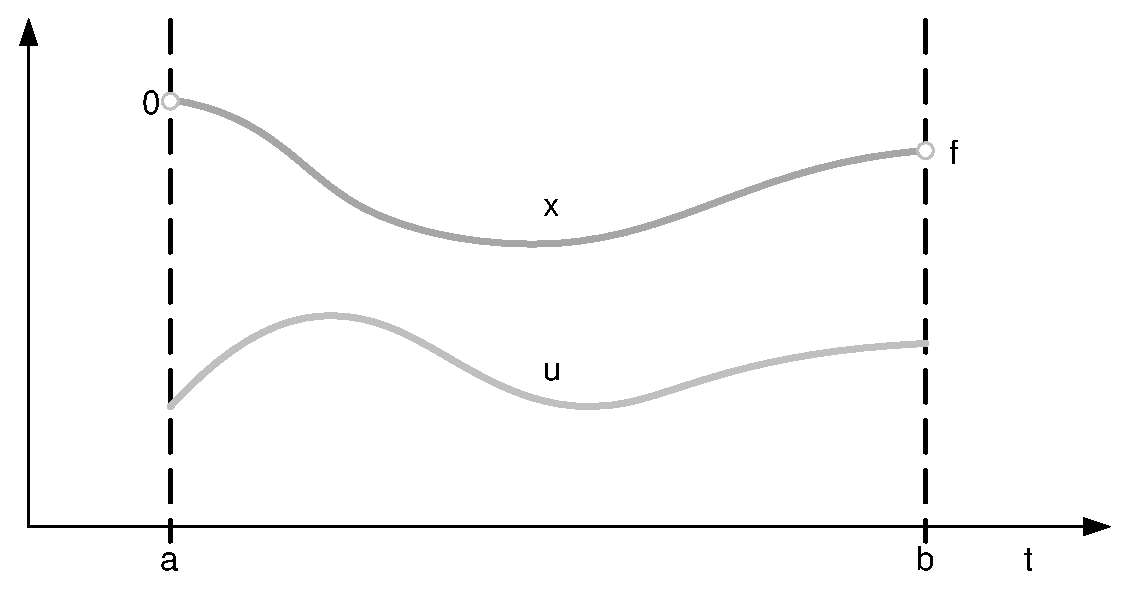
\includegraphics[width=0.5\textwidth,clip, trim = 0cm 0cm 0cm 0cm]{2_Darstellung_dynamische_Optimierung.eps}
%\hspace{.5cm}
 \includegraphics[width=1.0\textwidth,clip, trim = 0cm 0cm 0cm 0cm]{2_Darstellung_endliche_Parametrierung.eps}
	\caption[Endliche Parametrierung]{Endliche Parametrierung mittels abschnittsweise konstanter Eingänge \cite{papageorgiou2012optimierung}} 
	\label{fig:parametrisierte_nmpc}
\end{figure}
%
Der Systemeingang ist damit vollständig durch den (endlich-dimensionalen) Parametervektor $\bar{\bs{u}}$ beschrieben. Der Einfachheit halber wird im Folgenden eine feste Endzeit $t_f$ angenommen\footnote{Trifft das nicht zu, so ist der Optimierungsvektor um die Optimierungsvariable $t_f$ zu erweitern und die Wahl der Subintervallgrenzen im nichtlinearen Programm entsprechend dynamisch anzupassen.}. Eingesetzt in die Systemdynamik \eqref{equ:opt_systemdynamik} ergibt sich somit
\begin{align*}
	\dot{\bs{x}}(t) = \bs{f}(\bs{x}(t),\bs{\psi}(t,\bar{\bs{u}}),t), \quad &\bs{x}(t_0) = \bs{x}_0\; , 
\end{align*}
was ein Anfangswertproblem darstellt und auf dem Intervall $[t_0, t_f]$ mit gängigen ODE-Solvern\footnote{Methoden zur Lösung von gewöhnlichen Differentialgleichungen (\emph{ordinary differential equations}), beispielsweise \emph{Runge-Kutta}-Methoden \cite{Huckle2006,press2007numerical}.} gelöst werden kann. Es wird so die Trajektorie $\bs{x}(t) = \bs{\phi}(t,\bar{\bs{u}})$ erhalten. 

Des Weiteren ist gängige Praxis, die Einhaltung der Ungleichungsnebenbedingungen \eqref{equ:opt_ungleichungen} (nur) an den $N$ Subintervallgrenzen $t_i$ zu fordern (s.\ schwarze Punkte in Abb.\,\ref{fig:parametrisierte_nmpc}), was aufgrund des stetigen Zustandsverlaufs bei hinreichend vielen Subintervallen dazu führt, dass dazwischen die Nebenbedingungen nur unwesentlich verletzt werden können. \\
Insgesamt ergibt sich somit das statische Optimierungsproblem \cite{papageorgiou2012optimierung, graichen2014SkriptOpt}
\begin{subequations}
\begin{align}
	\underset{\bar{\bs{u}}}{\text{minimiere}}  \quad & %J(\bs{\phi}(t,\bar{\bs{u}}),\bs{\psi}(t,\bar{\bs{u}}),t)) = 
	\int_{t_0}^{t_f} l(\bs{\phi}(t,\bar{\bs{u}}),\bs{\psi}(t,\bar{\bs{u}}),t)\,{\rm d} t + V(\bs{\phi}(t_f,\bar{\bs{u}})) \\
	\text{u.B.v.} \quad &\bs{g}(\bs{\phi}(t_f,\bar{\bs{u}}),t_f) = \bs{0}\\ 	
	&\bs{h}(\bs{\phi}(t_i,\bar{\bs{u}}),\bs{\psi}(t_i,\bar{\bs{u}}))  \leq \bs{0},  \quad  i=0,\ldots,N \;. 
\end{align} 
\end{subequations}
Anschaulich gesprochen wird in Abhängigkeit von %einer Startlösung für 
$\bar{\bs{u}}$ die Systemdynamik in "`einem Schuss"' simuliert, was dem Verfahren seinen Namen gibt. Bei der Implementierung bietet sich an, hierbei gleich die laufenden Kosten $l$ für die Berechnung von \eqref{equ:opt_funktional} durch Erweiterung des Systemzustands zu integrieren. Im Anschluss werden dann das Kostenfunktional (streng genommen nun nur noch eine Kostenfunktion von $\bar{\bs u}$) sowie die Nebenbedingungsungleichungen und Endbedingungen evaluiert. Je nach eingesetztem statischen Optimierungsverfahren wird dieser Vorgang mit einer Variation von $\bar{\bs{u}}$ wiederholt, sodass darauf geschlossen werden kann, wie die Lösung zu verbessern ist, um zum Optimum zu konvergieren.

Da sich innerhalb der Optimierung in jedem Schritt die Zustandstrajektorie $\bs{x}(t)$ erst aus der Steuertrajektorie $\bar{\bs{u}}$ ergibt, wird das Verfahren als \emph{sequentiell} bezeichnet. Wird hingegen die Zustandstrajektorie gleichzeitig mit der Steuertrajektorie optimiert, wird von \emph{simultanen} Verfahren gesprochen. Eine der bekanntesten Vertreter sind Mehrfachschießverfahren, die nachfolgend dargestellt sind.

\subsection{Direkte Mehrfachschießverfahren\index{Mehrfachschießverfahren}} \label{sec:direkte_mehrfach_schiessverfahren}
Die Grundidee von \emph{direkten Mehrfachschießverfahren}, (\emph{direct multi shooting}, s.\ beispielsweise \cite{diehl_fast_multipleshooting, papageorgiou2012optimierung, graichen2014SkriptOpt}) ist, die Herangehensweise des vorangegangen Abschnitts dahingehend zu modifizieren, dass nunmehr auf jedem der $N$ Teilintervalle ein Anfangswertproblem der Art
\begin{align*}
	\dot{\bs{x}}_i(t) = \bs{f}(\bs{x_i}(t),\bs{\psi}(t,\bar{\bs{u}}),t), \quad &\bs{x}(t_i) = \bs{s}_i \quad \text{für} \quad t \in [t_i, t_{i+1})
\end{align*}
gelöst wird. Hierbei stellen die Variablen $\bs{s}_i$ zusammengefasst als $\bar{\bs{s}} = [\bs{s}_0, \bs{s}_1, \ldots, \bs{s}_{N-1}]^\T$ die Anfangszustände für die Teiltrajektorien $\bs{x}_i(t) = \bs{\phi}_i(t,\bs{u}_i,\bs{s}_i)$ eines jeden Subintervalls dar, s.\ Abb.\,\ref{fig:parametrisierte_nmpc_multi}, von denen aus \emph{jeweils} "`nach vorne geschossen"' wird. Damit am Ende der Optimierung die zusammengesetzte Gesamttrajektorie an den Übergängen stetig ist, muss dort zusätzlich die Nebenbedingung $\bs{s}_{i+1} = \bs{\phi}_i(t_{i+1},\bs{u}_i,\bs{s}_i)$  gefordert werden. Der Optimierungsvektor umfasst neben $\bar{\bs{u}}$ nun auch noch die Anfangszustände $\bar{\bs{s}}$, sodass daraus das statische Optimierungsproblem \cite{papageorgiou2012optimierung, graichen2014SkriptOpt}
\begin{subequations}
\begin{align*}
	\underset{\bar{\bs{u}}, \bar{\bs{s}}}{\text{minimiere}}  \quad & %J(\bs{\phi}(t,\bar{\bs{u}}),\bs{\psi}(t,\bar{\bs{u}}),t)) = 
	\sum_{i=0}^{N-1}{\int_{t_i}^{t_{i+1}}} l(\bs{\phi}_i(t,\bs{u}_i,\bs{s}_i),\bs{u}_i)\,{\rm d} t + V(\bs{\phi}_{N-1}(t_{N-1},\bs{u}_{N-1},\bs{s}_{N-1}))
\end{align*}
\begin{align*}
	\text{u.B.v.} \quad &\bs{g}(\bs{\phi}_{N-1}(t_{N-1},\bs{u}_{N-1},\bs{s}_{N-1})) = \bs{0}\\ 	
	&\bs{h}(\bs{s}_i,\bs{u}_i) \leq \bs{0},  & i&=0,\ldots,N \\
	&\bs{s}_0 - \bs{x}_0 = 0 \\
	&\bs{s}_{i+1} - \bs{\phi}_i(t_{i+1},\bs{u}_i,\bs{s}_i) = 0, & i&=0, \ldots,N-2
\end{align*} 
\end{subequations}
resultiert.
Die Optimierung erfolgt gleichzeitig für $\bar{\bs{u}}$ und $\bar{\bs{s}}$, sodass \emph{simultan} die Zustands- und Steuertrajektorie optimiert werden.
%
\begin{figure}[h]
\centering
	\psfrag{0}[cr][cr][1.0]{$\bs{x}_0$}
	\psfrag{1}[cb][cb][1.0]{$\bs{u}_0$}
	\psfrag{2}[cb][cb][1.0]{$\bs{u}_1$}
	\psfrag{3}[cb][cb][1.0]{$\bs{u}_2$}
	\psfrag{f}[cl][cl][1.0]{$\bs{x}(t_f)$}
	\psfrag{t}[ct][ct][1.0]{$t$}
	\psfrag{a}[ct][ct][1.0]{$t_0$}
	\psfrag{b}[ct][ct][1.0]{$t_f$}
	\psfrag{x}[cb][cb][1.0]{$\bs{x}^\ast(t)$}
	\psfrag{u}[cb][cb][1.0]{$\bs{u}(t) = \bs{\psi}(t,\bar{\bs{u}})$}
	%\psfrag{1}[c][c][1.0]{$t_1$}
	%\psfrag{2}[c][c][1.0]{$t_p=t_0+N\cdot\delta$}
	\psfrag{4}[c][c][1.0]{$\bs{s}_0$}
	\psfrag{5}[c][c][1.0]{$\bs{s}_1$}
	\psfrag{6}[c][c][1.0]{$\bs{s}_2$}
	\psfrag{7}[cl][cl][1.0]{$\bs{g}=0$}
	\psfrag{c}[c][c][1.0]{$\bs{s}_{i+1}=\bs{\phi}_i(t_{i+1},\bs{u}_i,\bs{s}_i)$}
	\psfrag{g}[c][c][1.0]{$\bs{s}_{i+1} \neq \bs{\phi}_i(t_{i+1},\bs{u}_i,\bs{s}_i)$}
	\psfrag{x}[c][c][1.0]{$x_0$}
 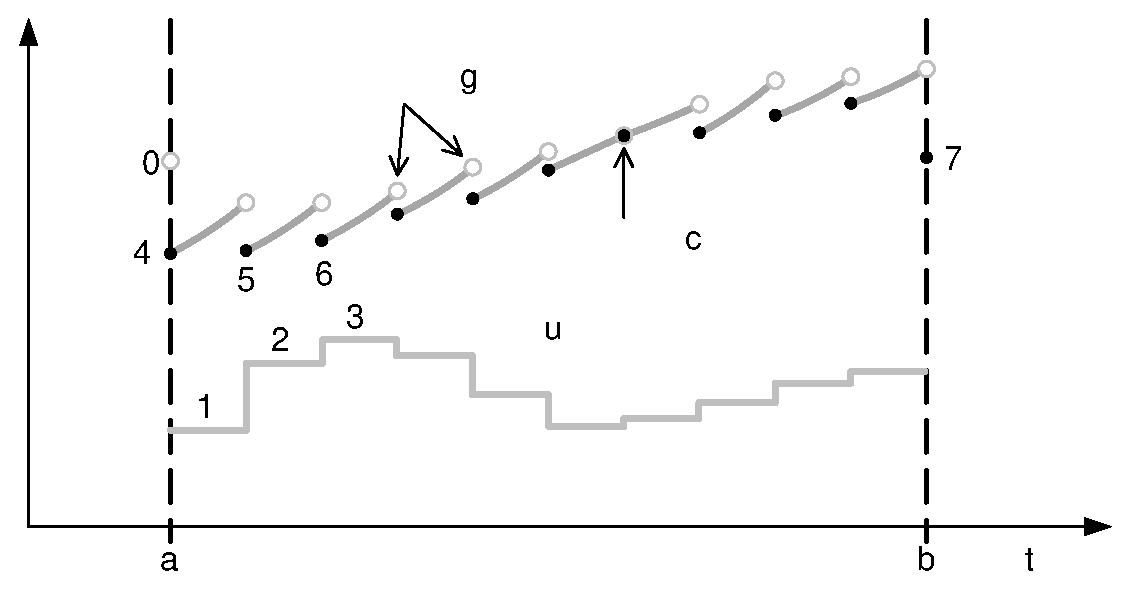
\includegraphics[width=1.0\textwidth,clip, trim = 0cm 0cm 0cm 0cm]{2_Multi_shooting.eps}
	\caption[Grundidee von Mehrfachschießverfahren]{Grundidee von Mehrfachschießverfahren \cite{diehl_fast_multipleshooting}}
	\label{fig:parametrisierte_nmpc_multi}
\end{figure}
%
Die Dimension des Optimierungsproblems ist somit gegenüber dem Einfachschießverfahren gestiegen, es weist aber eine dünn besetzte Struktur auf, die von einer ganzen Reihe statischer Optimierungsverfahren ausgenutzt werden kann \cite{diehl_fast_multipleshooting}. Des Weiteren wird aufgrund der Unabhängigkeit der Teilintervalle die Parallelisierung ihrer Evaluation auf mehrere Rechenkerne möglich, was eine erhebliche Rechenzeiteinsparung mit sich bringen kann (vgl.\ auch \cite{behrendt2011paralleles}). Der größte Vorteil besteht jedoch darin, dass sich für instabile und stark nichtlineare Systeme das Konvergenzverhalten stark verbessert \cite{diehl_numerical_methods}, da das Modell während der Optimierung auf den kurzen Intervallen nicht so weit "`abhauen"' kann.

Werden die Subintervalle auf einen einzigen Integrationsschritt reduziert, die Differentialgleichung also an den Stützstellen $\bs{s}_i$ diskretisiert (z.B. durch die Trapezregel), so wird auch von Volldiskretisierung gesprochen, welche im Rahmen der Trajektorienplanung z.B. in \cite{gerdts2009generating} zum Einsatz kommt.

%Übergang zu Volldiskretisierung, Überlegen, ob Kapitelaufteilung besser wenn "`Simultane"' und Sequentielle Verfahren?

	%[Graichen und Grüne]
%\begin{figure}[H]
	%\vspace{-0.3cm}
	%\psfrag{0}[c][c][1.0]{$t_0$}
	%\psfrag{1}[c][c][1.0]{$t_1$}
	%\psfrag{2}[c][c][1.0]{$t_{\text{horiz}}=t_0+N\cdot\delta$}
	%\psfrag{3}[c][b][1.0]{Optimierungshorizont $T_{\text{horiz}}$}
	%\psfrag{4}[c][c][1.0]{Vergangenheit}
	%\psfrag{5}[c][c][1.0]{\textbf{Prädiktion}}
  %\psfrag{a}[c][b][1.0]{Systemzustand x}
	%\psfrag{b}[c][c][1.0]{prädizierter Systemzustand $\bar{x}$}%{\textit{prädizierter Systemzustand} $\bar{x}$}
	%\psfrag{c}[c][b][1.0]{Stellgröße u}
	%\psfrag{d}[c][b][1.0]{Stellgrößensequenz $\{\bar{u}_k\}$}%{\textit{Stellgrößensequenz} $\{\bar{u}_k\}$}
	%\psfrag{u}[c][c][1.0]{$\bar{u}_1$}
	%\psfrag{w}[c][c][1.0]{$\bar{u}_2$}
	%\psfrag{v}[c][c][1.0]{$\bar{u}_N$}
	%\centering
 %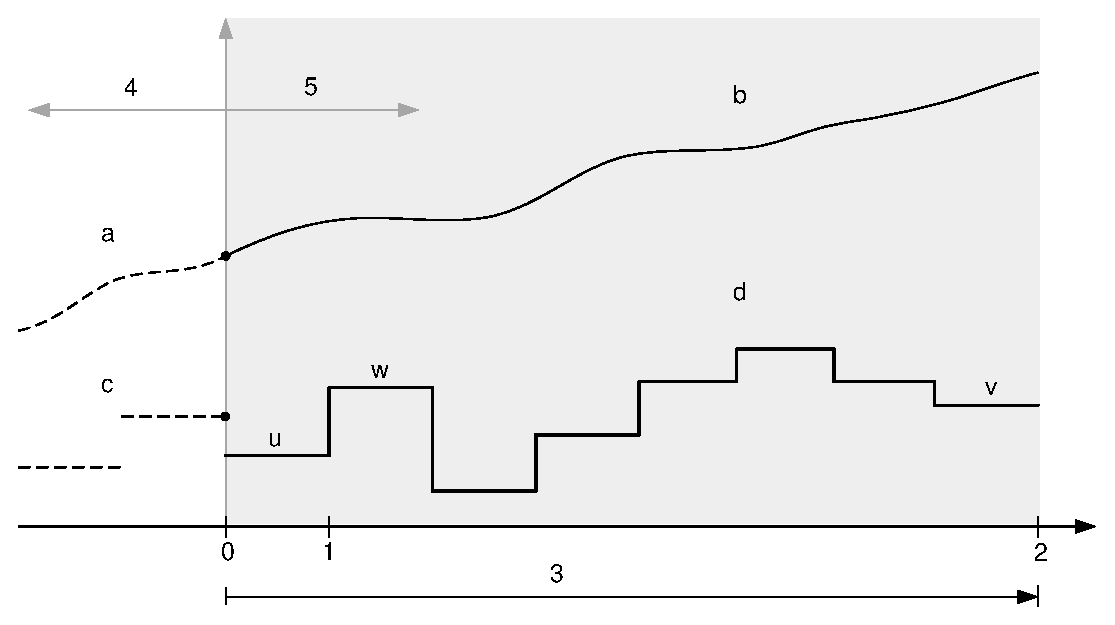
\includegraphics[width=0.99\textwidth,clip, trim = 0cm 0cm 0cm 0cm]{5_nmpc_parametrisierung.eps}
		%\ \vspace{-0.45cm}
	%\caption[Parametrisierte modellprädiktive Regelung]{Parametrisierte modellprädiktive Regelung, abgewandelte Darstellung nach \cite{Findeisen2002}}
	%\label{fig:parametrisierte_nmpc}
%\end{figure} 


	%\subsection{Diskretisierungsverfahren}
	%	\subsubsection{Teildiskretisierung}
	%	\subsubsection{Volldiskretisierung}

%\begin{figure}[H]
	%\psfrag{0}[c][c][1.0]{$t_0$}
	%\psfrag{1}[c][c][1.0]{$t_1$}
	%\psfrag{2}[c][c][1.0]{$t_p=t_0+N\cdot\delta$}
	%\psfrag{b}[r][c][1.0]{\textit{prädizierter Systemzustand} $\bar{x}=\bar{x}(t;\{\bar{u}_k\})$}
	%\psfrag{u}[c][c][1.0]{$\bar{u}_1$}
	%\psfrag{w}[c][c][1.0]{$\bar{u}_2$}
	%\psfrag{v}[c][c][1.0]{$\bar{u}_N$}
	%\centering
  	%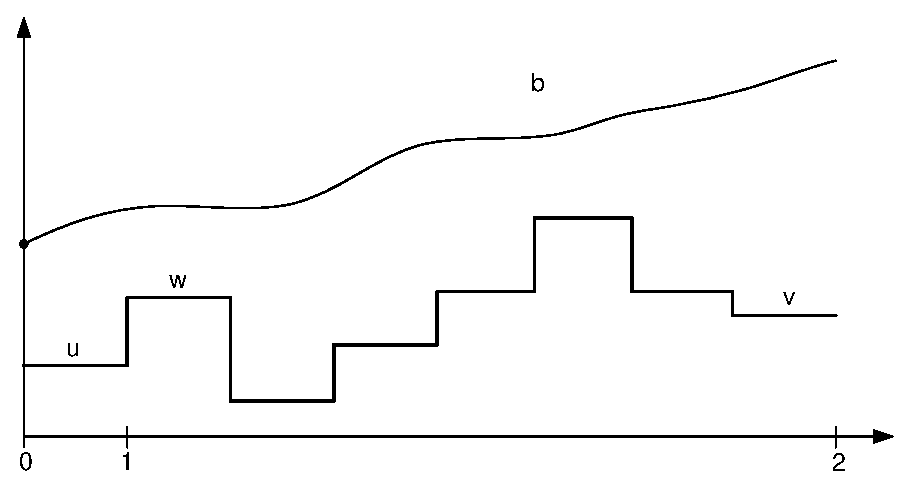
\includegraphics[width=0.98\textwidth,clip, trim = 0cm 0cm 0cm 0cm]{5_shooting_single.eps}
		%\vspace{0.3cm}
	%\caption[Darstellung der Grundidee von Single-Shooting]{Darstellung der Grundidee von Single-Shooting, abgewandelte Darstellung nach \cite{diehl_fast_multipleshooting}}
	%\label{fig:single-shooting}
	%\vspace{-0.2cm}
%\end{figure} 
		%

%\begin{figure}[H]
	%\psfrag{0}[c][c][1.0]{$t_0$}
	%\psfrag{1}[c][c][1.0]{$t_1$}
	%\psfrag{2}[c][c][1.0]{$t_p=t_0+N\cdot\delta$}
	%\psfrag{4}[c][c][1.0]{$s_0$}
	%\psfrag{5}[c][c][1.0]{$s_1$}
	%\psfrag{6}[c][c][1.0]{$s_2$}
	%\psfrag{7}[c][c][1.0]{$s_N$}
	%\psfrag{b}[c][c][1.0]{\textit{prädizierter Systemzustand} $\bar{x}_i(t_{i+1};s_i,\bar{u}_i)$}
	%\psfrag{c}[c][c][1.0]{$s_{i+1}=\bar{x}_i(t_{i+1};s_i,\bar{u}_i)$}
	%\psfrag{f}[c][c][1.0]{$s_{i+1}\neq\bar{x}_i(t_{i+1};s_i,\bar{u}_i)$}
	%\psfrag{u}[c][c][1.0]{$\bar{u}_1$}
	%\psfrag{w}[c][c][1.0]{$\bar{u}_2$}
	%\psfrag{v}[c][c][1.0]{$\bar{u}_N$}
	%\psfrag{x}[c][c][1.0]{$x_0$}
	%\centering
  	%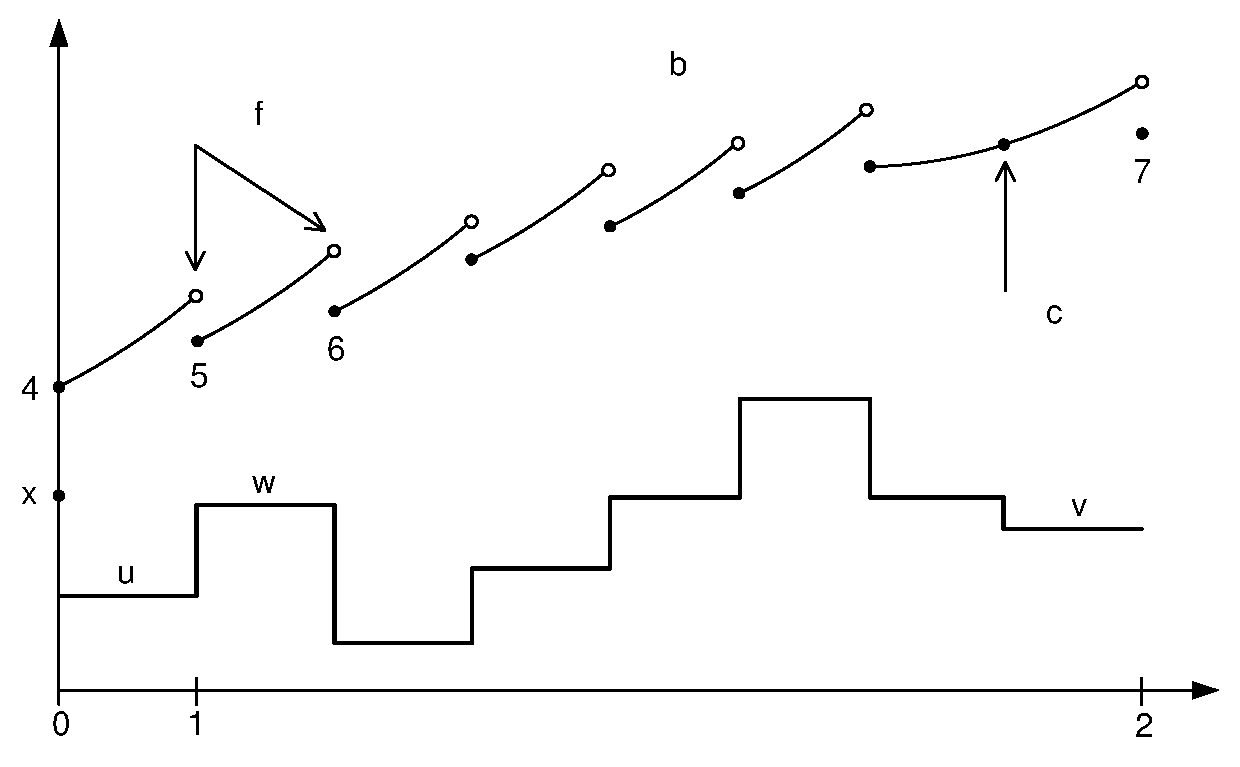
\includegraphics[width=0.98\textwidth,clip, trim = 0cm 0cm 0cm 0cm]{5_shooting_multi.eps}
	%\vspace{0.15cm}
	%\caption[Darstellung der Grundidee von Multi-Shooting]{Darstellung der Grundidee von Multi-Shooting, abgewandelte Darstellung nach \cite{diehl_fast_multipleshooting}}
	%\label{fig:multi-shooting}
%\end{figure} 



\subsection{Flachheitsbasierte Ausgangsparametrierung\index{Flachheit}} \label{sec:flachheitbasierte_para}
Anstelle der zuvor beschriebenen Parametrierung des Systemeingangs bietet sich bei der Klasse der sog.\ \emph{flachen} Systeme \cite{fliess1995fad} eine Parametrierung über einen geeigneten (fiktiven) Systemausgang an, den \emph{flachen} Ausgang. Da auch die Fahrzeugdynamik als flaches System formuliert werden kann \cite{rothfuss1997fnz, fuchshumer2005nvd}, wird zunächst die Flachheitseigenschaft definiert. 
Hierzu dient als Ausgangspunkt die nichtlineare Zustandsraumdarstellung
\begin{align} \label{equ:system_flach}
	\dot{\bs{x}} = \bs{f}(\bs{x},\bs{u}), \quad &\bs{x}(t_0) = \bs{x}_0 \in \mathbb{R}^n, \quad \bs{u}\in \mathbb{R}^m ,
\end{align}  
wobei vorausgesetzt wird, dass die Funktion $\bs{f}$ hinreichend oft stetig differenzierbar ist. 
\begin{mydef}
Ein nichtlineares System der Form \eqref{equ:system_flach} heißt (differentiell) flach\index{Flachheit} \cite{fliess1995fad}, wenn ein (fiktiver) Ausgang
\begin{align*}
	\bs{z} = \bs{\Phi}\left( \bs{x}, \bs{u}, \dot{\bs{u}}, \ldots, \bs{u}^{(\alpha)}\right)
\end{align*}
mit $\text{dim}\,\bs z = \text{dim}\,\bs u$ existiert\footnote{In der Praxis kann häufig ein flacher Ausgang gefunden werden, der nur eine Funktion des Zustands ist, d.h.\ $\bs{z} = \bs{\phi}( \bs{x})$.}, der folgende Bedingung erfüllt. Sowohl die Zustände $\bs{x}$ als auch die Eingänge $\bs{u}$ können als Funktionen von $\bs{z}$ und einer endlichen Anzahl seiner Zeitableitungen ausgedrückt werden, d.h.\
\begin{subequations} \label{equ:inverse_flach}
\begin{align} 
	\bs{x} &= \bs{\Psi}_x\left( \bs{z}, \dot{\bs{z}}, \ldots, \bs{z}^{(\beta-1)}\right) \\
	\bs{u} &= \bs{\Psi}_u\left( \bs{z}, \dot{\bs{z}}, \ldots, \bs{z}^{(\beta)}\right) \;.
\end{align}
\end{subequations}
\end{mydef}
Aufgrund von $\text{dim}\,\bs z = \text{dim}\,\bs u$ sind die Komponenten von $\bs{z}$ (differentiell) unabhängig voneinander \cite{rothfuss1997fnz}.

Im Hinblick auf die Optimierung mittels direkter Methode bietet sich nun der große Vorteil, dass durch \eqref{equ:inverse_flach} die Größen $\bs{x}$ und $\bs{u}$ durch den flachen Ausgang $\bs z$ ausgedrückt werden können, und die Differentialgleichung \eqref{equ:system_flach} des Systems nicht weiter berücksichtigt werden muss. Dementsprechend reicht es aus, eine endliche Parametrierung des Ausgangssignals 
\begin{align*}
	\bs{z}(t) = \bs{\psi}_z(t,\bar{\bs{z}}) \quad t\in[t_0, t_{f}]
\end{align*}
mit dem Parametervektor $\quad \bar{\bs{z}} = [\bs{z}_0, \bs{z}_1, \ldots]^\T$ zu finden, die sicherstellt, dass $\bs{z}(t)$ hinreichend oft stetig differenzierbar ist, etwa über Polynome \cite{zeitz2010differenzielle} oder Splines \cite{de2009flatness}. \\
Damit ergibt sich das statische Optimierungsproblem
\begin{subequations}
\begin{align} \nonumber
	\!\!\!\!\!\!\!\!\!\!\!\!\underset{\bar{\bs{z}}}{\text{minimiere}}  & %J(\bs{\phi}(t,\bar{\bs{u}}),\bs{\psi}(t,\bar{\bs{u}}),t)) = 
	\int_{t_0}^{t_f} \! l \!\left(\bs{\Psi}_x\!\left( \bs{\psi}_z(t,\bar{\bs{z}}), \dot{\bs{\psi}}_z(t,\bar{\bs{z}}), \ldots\right)\!,\bs{\Psi}_u\!\left( \bs{\psi}_z(t,\bar{\bs{z}}), \dot{\bs{\psi}}_z(t,\bar{\bs{z}}), \ldots\right)\!\right){\rm d} t \label{equ:kost_flach}\\
	&\quad + V\left(\bs{\Psi}_x\left( \bs{\psi}_z(t_f,\bar{\bs{z}}), \dot{\bs{\psi}}_z(t_f,\bar{\bs{z}}), \ldots\right)\!\right) \\
	\!\!\!\!\!\!\!\!\!\! \text{u.B.v.} \quad &\bs{g}\!\left(\bs{\Psi}_x\left( \bs{\psi}_z(t_f,\bar{\bs{z}}), \dot{\bs{\psi}}_z(t_f,\bar{\bs{z}}), \ldots\right)\!\right) = \bs{0}\\ 	
	&\bs{h}\!\left(\bs{\Psi}_x\!\left( \bs{\psi}_z(t_i,\bar{\bs{z}}), \dot{\bs{\psi}}_z(t_i,\bar{\bs{z}}), \ldots\right)\!,\bs{\Psi}_u\!\left( \bs{\psi}_z(t_i,\bar{\bs{z}}), \dot{\bs{\psi}}_z(t_i,\bar{\bs{z}}), \ldots\right)\!\right)  \!\leq \! \bs{0},  \nonumber \\
	& \quad i=1,\ldots,N.  \label{equ:nebenbedinungung_flach}
\end{align} 
\end{subequations}
Zur Evaluation des Kostenfunktionals $J$ in \eqref{equ:kost_flach} muss dann lediglich $l$ numerisch integriert werden; ein Lösen der Differentialgleichung \eqref{equ:system_flach}, wie in den Abschn.\,\ref{sec:direkte_einfach_schiessverfahren} und \ref{sec:direkte_mehrfach_schiessverfahren}, ist aufgrund der Ausnutzung der Flachheitseigenschaft nicht erforderlich, was zu einer erheblichen Rechenaufwandsreduktion führen kann. Zur Evaluation von \eqref{equ:nebenbedinungung_flach} müssen die Nebenbedingungen jedoch noch zusätzlich zu $N$ Zeitpunkten evaluiert werden, die hinreichend eng zu wählen sind, s.\ Abb.\,\ref{fig:flachheitsbasierte_optimierung}. \\
Aufgrund der flachheitsbasierten Systemparametrierung werden über den Ausgang $\bs{z}(t)$ gleichzeitig der Systemeingang $\bs{u}(t)$ und die Systemzustandsgrößen $\bs{x}(t)$ optimiert, sodass diese Herangehensweise zu den simultanen Verfahren zu zählen ist.
%\cite{ziegler_todo}


\begin{figure}[ht]
\centering
  \psfrag{0}[cr][cr][1.0]{$\bs{x}_0$}
	\psfrag{f}[cl][cl][1.0]{$\bs{x}(t_f)$}
	\psfrag{z}[cb][cb][1.0]{$\bs{z}(t) = \bs{\psi}_z(t,\bar{\bs{z}})$}
	\psfrag{7}[cl][cl][1.0]{$g=0$}
	\psfrag{t}[ct][ct][1.0]{$t$}
	\psfrag{a}[ct][ct][1.0]{$t_0$}
	\psfrag{b}[ct][ct][1.0]{$t_f$}
	\psfrag{c}[ct][ct][1.0]{$t_1$}
	\psfrag{e}[ct][ct][1.0]{$t_2$}
	\psfrag{x}[lt][lt][1.0]{$\bs{x}(t) = \bs{\Psi}_x\!\left( \bs{\psi}_z(t,\bar{\bs{z}}), \dot{\bs{\psi}}_z(t,\bar{\bs{z}}), \ldots\right)$}
	\psfrag{u}[lt][lt][1.0]{$\bs{u}(t) = \bs{\Psi}_u\!\left( \bs{\psi}_z(t,\bar{\bs{z}}), \dot{\bs{\psi}}_z(t,\bar{\bs{z}}), \ldots\right)$}
 %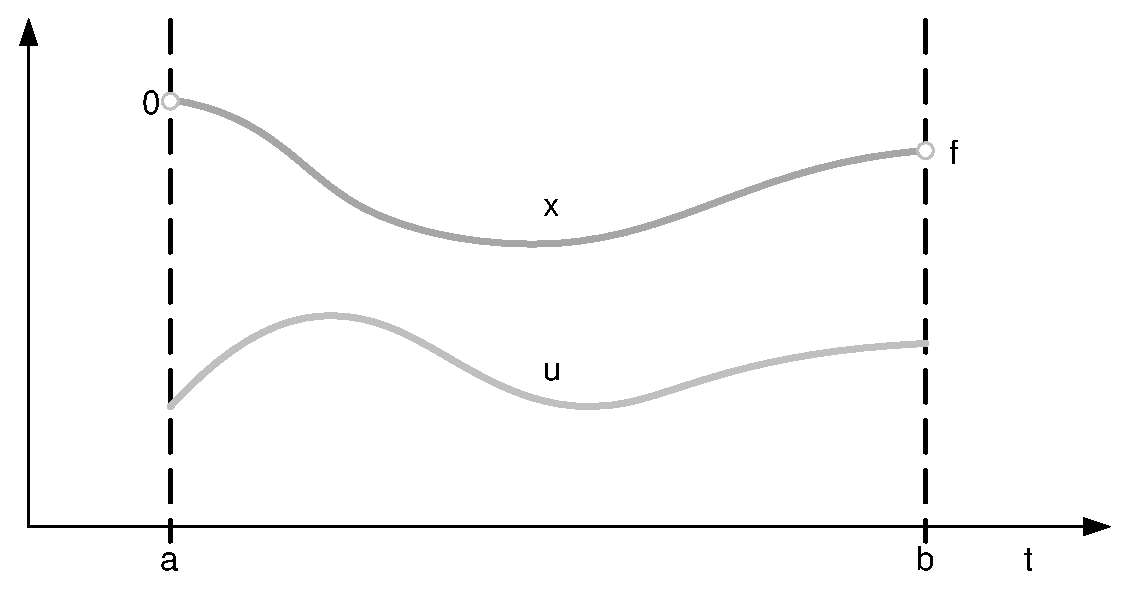
\includegraphics[width=0.5\textwidth,clip, trim = 0cm 0cm 0cm 0cm]{2_Darstellung_dynamische_Optimierung.eps}
%\hspace{.5cm}
 \includegraphics[width=1.0\textwidth,clip, trim = 0cm 0cm 0cm 0cm]{2_Darstellung_flachheitsbasierte_optimierung.eps}
	\caption[Endliche Parametrierung durch flachen Ausgang]{Endliche Parametrierung des gesamten Systemverhaltens durch flachen Ausgang $\bs{z}(t)$} 
	\label{fig:flachheitsbasierte_optimierung}
\end{figure}

%\section{Problemformulierung für die Fahrzeuganwendung}
% Erst adhoc-Herangehensweise mit sigmoid und co.

% Idee für andere Kapitel:
% - Dynam. Progr. --> 
% Systembeschreibung: verweis auf direkte Optimierung, zum Verbinden der Knoten (dann typischerweise: maximale Krümmung, stetiger Krümmungsverlauf)
% Endbedingungen und Ungleichungsbeschränkungen: Entlang der Straße, Querablage aber frei, oder: Zielpose def. durch Parkplatz
% Fokus auf Kollisionscheck, also x,y,psi (Ausnahme Ziegler Boppardslides)

% Literatur:

%\cite{Falcone2007} % DM Fahrzeugregelung
%\cite{Yoon2009} % DM, PP
%\cite{preusse2001fahrzeugfuhrung} % DM, PP, at, Fahrbahnfestes Koordinatensystem

%\cite{gerdts2009generating} % DM, EP, offline
%\cite{kelly2003reactive} % DM, PS
%\cite{park2009obstacle} % DM, PP

%\cite{anderson2010optimal} 	% DM, PP
%\cite{bohren2008little}			% DM, PP

%\cite{schmidt2012hierarchischer} % DM, Bahnplanung (Rennstrecke
%\cite{Konig2008} % NMPC für Rundenzeitplanung
% nicht zitiert \cite{tentacels08} 	% Kreisbögen, DM, PP -> nicht führ höhere Geschwindigkeiten gedacht
\section{Fahrzeugspezifische Problemformulierungen}
\subsection{Systembeschreibung} \label{sec:direkte_methode_systembeschreibung}
Grundsätzlich eignet sich für die direkte Optimierungsmethode jedes Systemmodell, das sich numerisch stabil simulieren lässt und die im Kostenfunktional \eqref{equ:opt_funktional} verwendeten Systemzustände $\bs x$ umfasst. Dennoch gilt auch hier die Devise: \emph{So einfach wie möglich, so genau wie nötig!} Aufgrund der  Arbeitsweise des nichtlinearen Programms wird nämlich in jedem Iterationsschritt die numerische Simulation des Modells viele Male durchgeführt und beansprucht damit den Großteil der Rechenzeit der direkten Optimierung. Für eine effiziente Simulation lohnt sich in jedem Fall der Blick auf die laufenden Kosten $l$ in \eqref{equ:opt_funktional}, welche  Aufschluss darüber geben, wie durch eine geeignete Systemkoordinatenwahl aufwändige Funktionsevaluationen zu vermeiden sind. Ein Beispiel hierfür stellt die Optimierung der Fahrzeugbewegung entlang der Straße dar. Dabei interessiert nicht der Fahrzeugabstand vom Koordinatenursprung sondern vielmehr die Fahrzeugposition innerhalb der Spur, sodass die Fahrzeugbewegung, wie in \cite{preusse2001fahrzeugfuhrung, schmidt2012hierarchischer}, direkt in den sog.\ \emph{Frénet-Koordinaten}\index{Frénet-Koordinaten} der Straße modelliert wird (s.\ hierzu später auch Abschn.\,\ref{sec:nmpc_beispiel}). \\
Da das optimierte Manöver vom Fahrzeug abgefahren werden muss, ist es wichtig, dessen Dynamik in der Systembeschreibung zu berücksichtigen, unabhängig davon, welcher Systemteil von einer unterlagerten Regelung stabilisiert wird.  Hierbei ist es hilfreich zu wissen, dass über den Lenkwinkel $\delta$ (bei Vernachlässigung der Reifeneinlauflängen \cite{mitschke2004dynamik}) direkt die Reifenquerkräfte beeinflusst werden und damit auch ein unmittelbarer Zusammenhang zur Fahrzeugquerbeschleunigung $a_q$ und Kurskrümmung $\kappa$ besteht. Während es für langsame Manöver (Einparken, z.B.\ \cite{kelly2003reactive}) oder schnelle Manöver mit gleichmäßigen Lenkbewegungen wie auf der Rennstrecke (z.B.\ \cite{Konig2008, gerdts2009generating}) ausreicht, stetige Krümmungen \bzw Querbeschleunigungen zu generieren, adressieren Notfallmanöver das instationäre Fahrverhalten, sodass weitere Fahrzeugzustände wie der Schwimmwinkel $\beta$ und die Gierrate $r$ zu berücksichtigen sind 
\cite{Falcone2007, park2009obstacle, schmidt2012hierarchischer, Yoon2009, nanao2011vehicle}. 
Gerade dann erweist sich die direkte Optimierungsmethode als äußerst vorteilhaft, da zudem auch Reifennichtlinearitäten 
\cite{gerdts2009generating, Yoon2009} oder gar dynamische Radlasten \cite{Falcone2007, Frasch2013b}
sowie umfangreiche Aktorikmodelle berücksichtigt werden können. Das gilt insbesondere bei einer Offline-Optimierung (z.B. Berechnung der Ideallinie auf einer Rennstrecke \cite{gerdts2009generating}), bei der die Rechenzeit eine untergeordnete Rolle spielt.
% TODO: Jakobimatrix analytisch!

% Vorteil: Änderungen in der Strecke, die z.B. bei der indirekten Methode große Änderungen nach sich ziehen, führen hier oft nur zu marginalen Änderungen im Programm
\subsection{Kostenfunktional\index{Kostenfunktional}} \label{sec:direkte_methode_kostenfuktional}
Im Kostenfunktional ist, wie zuvor beschrieben, genau das ungewollte Systemverhalten mit Kosten zu belegen, sodass bei der Optimierung dieses minimiert wird. Hierzu zählen vor allem Kurskrümmungs-, Querbeschleunigungs- oder Lenkwinkeländerung
\cite{anderson2010optimal,Liu2010}
(je nach Modellierung der Systemzustände oder -eingänge), da sie zu einer unkomfortablen Fahrweise führen, die zudem nur mit großem Stellaufwand und Verschleiß von der Lenkaktorik umgesetzt werden kann. Bei Notmanövern bietet sich darüber hinaus an, die Annäherung an die fahrphysikalische Grenze zu bestrafen, indem die Beschleunigungen und der Schwimmwinkel in die Kosten eingehen
\cite{park2009obstacle, anderson2010optimal}. 
Schließlich kann auch die Straßenverkehrsordnung in der Form berücksichtigt werden, dass Abweichungen (und deren zeitliche Ableitungen) von der Straßenmitte 
\cite{park2009obstacle, Liu2010, nanao2011vehicle} zu den Gesamtkosten beitragen. In der Praxis wird das ungewollte Systemverhalten in aller Regel mit quadratischen Kostentermen beschrieben
\cite{Falcone2007,Yoon2009,park2009obstacle,anderson2010optimal,schmidt2012hierarchischer,Liu2010}, sodass sich die Integral- und Endkosten zu
\begin{align*}
l(\bs x(t), \bs u(t)) &= \bs x(t)^\T \bs Q \bs x(t) + \bs u(t)^\T \bs R \bs u(t) \\
V(\bs x(t_f)) &= \bs x(t_f)^\T \bs S \bs x(t_f)
\end{align*}
mit positiv definiten Wichtungsmatrizen $\bs Q$ und $\bs R$ ergeben. \\
% auch Zeitoptimalität
Im Hinblick auf die Systemsicherheit nimmt die Berücksichtigung anderer Verkehrsteilnehmer und weiterer Hindernisse einen zentralen Punkt bei der Optimierung ein. Auf den ersten Blick erscheint es zweckmäßig, die Fahrzeugannäherung an ein Objekt über der Zeit zu bestrafen und deshalb innerhalb der Integralkosten $l$ zu berücksichtigen. Das hat dann aber unweigerlich zur Folge, dass ein Manöver das Hindernis bei zunehmender Geschwindigkeit immer knapper passiert, da aufgrund der immer kürzeren Integrationszeit die Kosten fortwährend geringer ausfallen und die Optimierung zunehmend zugunsten einer geringeren Querbeschleunigung entscheidet. Da das dem subjektiven Risikoempfinden der Verkehrsteilnehmer widerspricht, empfiehlt sich die Erweiterung des Kostenfunktionals um sog.\ Punktkosten $\tilde V(\bs{x}(t_i),t_i)$ (welche in der Sonderform der Endkosten $V(\bs{x}(t_f),t_f)$ bereits in \eqref{equ:opt_funktional} aufgeführt sind), vgl.\ \cite{Liu2010}. Über sie können definierten Zeitpunkten $t_i$ bestimmte Kosten zugeschrieben werden. Um die Optimierung dazu zu bringen, einem Hindernis auszuweichen, muss demnach zunächst der Zeitpunkt bestimmt werden, an dem sich das Fahrzeug dem Hindernis am nächsten befindet. Abhängig von dem dann vorliegenden Abstand errechnen sich die Punktkosten, welche entsprechend hoch gewichtet werden müssen, um ein Schneiden des Hindernisses zu vermeiden, s.\ später Abschn.\,\ref{sec:costs_obstacles}.



%park2009obstacle
% Systemmodell: Lineares Einspurmodell
% Kostenfunktional: Zustände des ESM von Referenz --> Straße, Schwimmwinkel, 
% Nebenbedingungen: Querbeschleunigung über Radius beschränkt, Lenkwinkel
% Straße: Nur als linie
% Hindernisse: Parallaxe

%schmidt2012hierarchischer
% Systemmodell: Lineares Einspurmodell mit Seitenkraftsättigung
% Mist...





% Integralkosten, End- und Punktkosten, t_f, ICS

% nicht als nebenbedingungen, da Singularitäten.
% Dynamische Hindernisse problemlos möglich

\subsection{Nebenbedingungen\index{Nebenbedingungen}} \label{sec:direkte_opt_nb}% {Endbedingungen und Ungleichungsbeschränkungen}
Die Berücksichtigung von Nebenbedingungen in der Optimierung in Form von Gleichungs- oder Ungleichungsbeschränkungen ist ein probates Mittel, um wichtigen Systemeigenschaften Rechnung zu tragen, die nicht in der Differentialgleichung \eqref{equ:opt_systemdynamik} berücksichtigt sind, vgl.\ \cite{habilgroell}. Beim Fahrzeug zählt hierzu beispielsweise die konstruktionsbedingte Lenkwinkelbeschränkung. Im Unterschied zu den Optimierungskosten, über die mittels Wichtungsfaktoren Kompromisse zwischen konkurrierenden Optimierungszielen gefunden werden können (z.B.\ Komfort vs.\ Sicherheit bei einem Notmanöver), müssen die Nebenbedingungen zwingend eingehalten werden. Bei der dynamischen Neuplanung, die auf äußere Störungen und Kursänderungen anderer Verkehrsteilnehmer reagieren muss, bleibt es da nicht aus, dass ein sorgloser Umgang mit Nebenbedingungen \eqref{equ:opt_ungleichungen} dazu führt, dass diese zumindest kurzzeitig im Widerspruch zur Systemdynamik \eqref{equ:opt_systemdynamik} stehen. Aus der modellprädiktiven Regelung ist bekannt, dass eine (aktive) Nebenbedingung dazu führt, dass die Optimierungskosten immer weiter in den Hintergrund treten je näher (zeitlich gesehen) sie an den aktuellen Zeitpunkt herankommt, bis sie schließlich zu einer Singularität führt \cite{foellingeroptimal}. \\
Darum ist es von Vorteil, die Kollisionsfreiheit eines Manövers nicht als Nebenbedingung zu formulieren, sondern, wie zuvor beschrieben, die Annäherung an ein Hindernis in den Kosten zu berücksichtigen. Der Kostenterm für die Annäherung ist dann auf der einen Seite so auszulegen, dass selbst in der unmittelbaren Umgebung eines Hindernisses die restlichen Kosten einen wesentlichen Einfluss auf die Lösung haben, sodass das Fahrzeug dann nicht "`nervös"' zu lenken oder zu bremsen beginnt. Auf der anderen Seite dürfen die Kosten aber auch nicht so niedrig gewählt werden, dass das Manöver bereits in großer Entfernung vom Hindernis ein zukünftiges Schneiden in Kauf nimmt. \\ 
Die Berücksichtigung von Nebenbedingungen in den Optimierungskosten ist zwar formal immer möglich\footnote{Bestimmte statische Optimierungsverfahren behandeln grundsätzlich Nebenbedingungen über zusätzliche Kostenterme (sog.\ Penalty-Terme), s.\ z.B.\ \cite{papageorgiou2012optimierung, nocedal2006numerical}.}, führt jedoch bei einigen statischen Optimierungsverfahren erfahrungsgemäß zu einem erhöhten Rechenaufwand. Es bietet sich deshalb an, zumindest eingangsnahe Restriktionen (z.B. für den Lenkwinkel) als Nebenbedingungen in der Optimierung zu belassen, wenn sichergestellt ist, dass die von den Restriktionen betroffenen Systemzustände weder durch Störungen (aufgrund einer nachgelagerten Regelung, s.\ Abschn.\,\ref{sec:sys_stab}) noch von sich ändernden Umgebungsbedingungen (allen voran die Hindernisprädiktion) betroffen sind\footnote{Dennoch ist es erforderlich, numerisch-bedingte Singularitäten im Programm abzufangen, in dem z.B.\ die betroffenen Anfangszustände geringfügig korrigiert werden, sodass die Nebenbedingung eingehalten werden kann.}.   \\



% Nebenbdingungen haben dennoch ihre daseinsberechtigung: 
% 	- Direkte Methode wird immer auf Endlichem Horizont durchgeführt --> Endbedingungen um den Horizont zu erweitern
%   - Nebenbeingungen können in dem Systemteil verwendet werden, der durch einen folgeregler stabilisiert wird (fußnote: bei numerischen Schwierigkeiten muss getrixt werden) UND der zeitinvariant ist. (z.B. Lenkwinkelbeschränkung, Lenkratenbeschränkung, Bremsgradienten)




% geeignet für passierbereich, s. unten
% einschl. t_f
% ICS
% Diskretiersierung um Lösungsraum einzuschränken (Target manifolds)
% Ungleichungsbeschränkungen schlecht, weil hindernisse sich bewegung und es dadurch zu singularitäten kommen kann

%\subsection{Erweiterung des Kostenfunktionals um Punktkosten}
% mit Motivation zu Punktkosten
% Geeignet, wenn der Teil der von der Nebenbedingung betroffen ist, sich im simulierten Ersatzsystem befindet und nicht durch äußere Umstände/Signale beeinfluss werden kann (Ünderung der Kursrichtung)


% Modell: Entweder nur Fahrzeug oder Fz + andere (nicht steuerbare Verkehrsteilnehmer, Spurmarkierungen), kooperative Manöver
% Kostenfunktional erläutern, Integralkriterium: Energie, zeit-, quadratische Zustnadsgewichtung
% Überleitung Punktkosten: Erklärung über Gefahr von anderen Hindernissen
% Straße als ziel oder beeinflusst durch kosten, Frenet erklären

% S. auch Föllinger Seite 18 letzter Abschnitt, Tschebyscheff-Polynome: Funktional-> Funktion

% NMPC als rpp tool für maßgeschneiderten Algorithmus oder Offline-Optimierung mit Kombination mit Lattice Planner

% Vorwärtssimulation"'

% Einmalplaung (EP) Permanente Planung (PP)
% Direkte Methode (DM), Indirekte Methode (IM), dynamische Programmierung (DP)
% Trajektorienklasse

%Inhalte hiervon nehmen: \cite{diehl_fast_multipleshooting}


%\section{Online Implementierung}
%\cite{albersmeyer} % Fahrzeugregelung mit Real-time iterations und Verbesserungen

\section{Neuer Algorithmus für den aktiven Fußgängerschutz\index{Fußgängerschutz}} \label{sec:nmpc_beispiel} 
%
% Paper nur statt Fußgänger Ausweichen auf Autos (die sich nicht Querbewegen und somit die Situation verschärfen)
%	\section{Einleitung}
%
\zitat{Ein Fußgänger ist ein glücklicher Autofahrer, \\
	der einen Parkplatz gefunden hat.}{Joachim Fuchsberger}

Zur Verdeutlichung der konkreten Vorgehensweise bei der direkten Optimierungsmethodik wird eine Sicherheitsfunktion für den aktiven Fußgängerschutz herangezogen, die bereits in den im Rahmen der Arbeit entstandenen Veröffentlichungen \citeltex{werling2012walting, werling2012cdc} vorgestellt wurde. Aus Gründen der Einfachheit wird hier nur die Lösung des Optimalsteuerungsproblems erläutert, nicht jedoch der kontinuierliche Echtzeit-Betrieb, der geringfügige Modifikationen erfordert.

%Wie in der Einleitung erwähnt wurde, kann in den letzten Jahren eine deutliche Zunahme von Fahrerassistenzfunktionen in Serienfahrzeugen im Bereich der aktiven Sicherheit verzeichnet werden. 
Als Hintergrundinformation sei an dieser Stelle angemerkt, dass bereits heute in einigen Fahrzeugmodellen bei einer drohenden Fußgängerkollision eine automatische Notbremsung eingeleitet wird. Häufig verbleibt jedoch zu wenig Bremsweg zwischen Fahrzeug und Fußgänger, weshalb damit lediglich die Folgen einer Kollision reduziert werden können. %\cite{breuer2007real}. 
Durch eine zusätzliche automatische Fahrzeugausweichbewegung innerhalb der Fahrspur lässt sich in vielen Situationen dennoch eine Kollision vermeiden \cite{hattori2006optimum}. Mit der hierzu notwendigen Planung einer kombinierten Brems-Ausweich-Trajektorie gehen jedoch mehrere Herausforderungen einher, und zwar
\begin{itemize}
	\item die Berücksichtigung der prädizierten Fußgängerbewegung, 
	\item die nichtlinearen Kopplungseffekte der Fahrzeuglängs- und -querdynamik sowie
	%\item die Realisierung kurzer Planungszyklen sowie
	\item die Minimierung der durch das Ausweichmanöver hervorgerufenen Fahrerirritation,
\end{itemize}
welchen nachfolgend mit der Anwendung der direkten Optimierung begegnet wird.

%welche bereits erste Anwendungen im Bereich der Fahrzeugsicherheit gefunden hat, s.\ hierzu bspw.\ \cite{Liu2010, nanao2011vehicle}. \\

%Hierzu wird in Abschn.\,\ref{sec:modeling}
%ein Streckenmodell eingeführt, welches die vereinfachte Fahrzeugdynamik entlang einer Referenzkurve beschreibt. Anschließend muss dieses in Abschn.\,\ref{sec:constraints}
%um zusätzliche Restriktionen erweitert werden, die den fahrphysikalischen Grenzen Rechnung tragen. Ferner wird in Abschn.\,\ref{sec:costs} ein Kriterium formuliert, anhand dessen die Ausweichtrajektorie später zur Programmlaufzeit optimiert werden soll. Darauf aufbauend beleuchtet Abschn.\,\ref{sec:implementation} die Implementierung der Online-Trajektorienplanung als sog.\ Sequentielles Quadratisches Programm (SQP), welches schließlich seine Leistungsfähigkeit in Abschn.\,\ref{sec:results} anhand einer realitätsnahen Fußgänger-Fahrzeug-Simulation unter Beweis stellt. Der Beitrag schließt mit einer Zusammenfassung in Abschn.\,\ref{sec:conclusion}.

\subsection{Systemmodellierung}\label{sec:modeling}
Wesentlicher Inhalt der Manöverplanung ist das prädizierte Verhalten des Streckenmodells, welches damit das wichtigste Element der Trajektorienoptimierung darstellt, vgl.\ \cite{rawlings2000tutorial}. Aus Gründen der Robustheit wird allerdings die zur optimierten Ausweichtrajektorie berechnete Stellgröße nicht direkt der Fahrzeugaktorik zugeführt, sondern entsprechend Abschn.\,\ref{sec:sys_stab} an einen unterlagerten Regler als Sollvorgabe weitergeleitet. Das hat zur Folge, dass es reicht, die Lösung des Optimalsteuerungsproblems nicht ganz so häufig zu berechnen (z.B.\ mit $\unit[10]{Hz}$), ohne dass die Stabilität des Gesamtsystems gefährdet wird. Zusätzlich kann das Prädiktionsmodell zugunsten eines schnellen Optimierungsprozesses vereinfacht werden, da es geringeren Anforderungen genügen muss als das Reglerentwurfsmodell, welches die reale Stellgröße berechnet, s.\ Abschn.\,\ref{sec:sys_stab}.
%
Der erste Teil des Prädiktionsmodells stellt sich nun folgendermaßen dar, 
%With this in mind, we propose the first part of our prediction model,
\begin{subequations} \label{equ:dgl_mdl_nmpc}
\begin{align}
\label{equ:xdot}
\dot x_1 &= v \cos \theta \\
\dot x_2 &= v \sin \theta \\
\label{equ:thetadot}
\dot \theta &= \frac{v}{l \left[ 1 + \left[\frac{v}{v_{\text{ch}}}\right]^2\right]} \delta \\
\dot \delta &= u_1 \\ % \left[ 1 + \left[\frac{v}{v_{\text{ch}}}\right]^2 \right] \frac{l}{v^2}  u \\
\label{equ:vdot}
\dot v &= u_2.
\end{align}
\end{subequations}
Wie Abb.\,\ref{fig:systemStates} zu entnehmen ist, sind $x_1, x_2$ und $v$ die Fahrzeugreferenzposition und -ge\-schwin\-dig\-keit, $\theta$ bezeichnet die Kursrichtung und $\delta$ den (nicht dargestellten) Lenkwinkel der Reifen. Die Lenkwinkelrate wie auch die Zeitableitung der Geschwindigkeit dienen als Systemeingänge $u_1$ und $u_2$. Hierbei entstammt \eqref{equ:thetadot} der stationären Gierdynamik 
%\cite{allen1987steady} 
des linearen Einspurmodells (s.\ \zB \cite{mitschke2004dynamik, Heissing2008, Schramm2010}), dessen wichtigster Parameter die sog.\ charakteristische Geschwindigkeit
 $v_{\text{ch}} = \sqrt{[l^2  c_f c_r]/[m [c_r l_r - c_f l_f]]} $
ist. Sie hängt von der Fahrzeugmasse $m$, den Reifensteifigkeiten $c_f$ und $c_r$ sowie den Schwerpunktabständen $l_f$ und $l_r$ der Vorder- und Hinterachse als auch deren Gesamtabstand $l=l_f + l_r$ ab.

\begin{figure}%
\centering
\begin{minipage}{0.45\textwidth}%
\psfrag{1}[tc][tc][1.0]{$s_r$}
    \psfrag{2}[rb][rb][1.0]{$\kappa_r(s_r)$}
    \psfrag{3}[lb][lb][1.0]{$d_r$}
    \psfrag{4}[rb][rb][1.0]{$[x_1, x_2]$}
    \psfrag{5}[lt][lt][1.0]{$v$}
    \psfrag{6}[c][c][1.0]{$\theta$}
    \psfrag{7}[lt][lt][1.0]{$\theta_r$}
    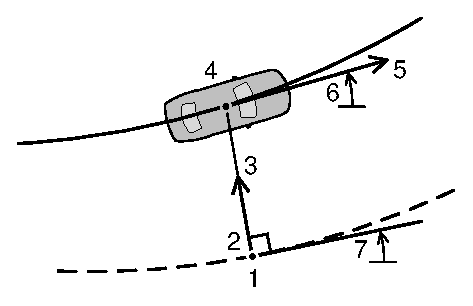
\includegraphics[width=1.0\textwidth,clip, trim = 1.5cm 0cm 0cm 0cm]{5_vehicleAndReferenceCurveStates.eps}
    \caption[Fahrzeugdynamik entlang einer Referenzkurve]{Systemzustände des vereinfachten Fahrzeugmodells entlang einer Referenzkurve \citeltex{werling2012cdc}}
    \label{fig:systemStates}
\end{minipage}%
\qquad
\begin{minipage}{0.45\textwidth}%
    \psfrag{1}[rb][rb][1.0]{$a_t$}
    \psfrag{2}[cb][cb][1.0]{$a_n$}
    \psfrag{3}[lc][lc][1.0]{$c_t$}
    \psfrag{4}[ct][ct][1.0]{$c_n$}
    \includegraphics[width=1.0\textwidth,clip, trim = 0cm 0cm 0cm 0cm]{5_KammscherKreis}
    \caption[Elliptische Näherung der zulässigen Fahrzeugbeschleunigung]{Elliptische Näherung der zulässigen Gesamtfahrzeugbeschleunigung \citeltex{werling2012cdc}\index{Kamm'scher Kreis}s}
    \label{fig:kammscherKreis}
\end{minipage}%
\end{figure}%

Das Modell bietet zwei große Vorteile gegenüber dem gewöhnlichen Einspurmodell. Zum einen ist es für $v=0$ singularitätsfrei und ermöglicht dadurch eine Bremsung bis in den Stillstand. Zum anderen sind dessen Differentialgleichungen nicht sonderlich steif, was eine verhältnismäßig große numerische Simulationsschrittweite mit erheblich reduziertem Rechenaufwand ermöglicht. Um den unterlagerten Regelkreis während der extremen Fahrmanöver nicht zu überfordern, müssen der Trajektorie allerdings zusätzliche Restriktionen wie die vom Fahrzeug maximal erreichbare Querbeschleunigung auferlegt werden, was in Abschn.\,\ref{sec:constraints} erfolgt. \\
%
Als Wegbereiter für eine effektive Evaluation der Trajektoriengüte, s.\ auch Absch.\,\ref{sec:direkte_methode_systembeschreibung}, wird zusätzlich die Dynamik der Projektion des Fahrzeugs auf eine Referenzkurve (z.B.\ die Fahrstreifenmitte) modelliert, s.\ schwarzer Punkt auf gestrichelter Linie in Abb.\,\ref{fig:systemStates}. Hierbei stellen die Kursrichtung $\theta_r$, der vorzeichenbehaftete Abstand $d_r$ zum Fahrzeug, und die zurückgelegte Wegstrecke $s_r$ der Projektion die Systemzustände dar. Mit Hilfe der Differentialgeometrie \cite{morin2008hrc} lässt sich unter Berücksichtigung der Referenzkurvenkrümmung $\kappa_r(s_r)$ das bestehende Modell  \eqref{equ:dgl_mdl_nmpc} um die Differentialgleichungen
\begin{subequations} \label{equ:dgl_mdl_nmpc_2}
\begin{align}
\label{equ:d_r_dot}
\dot d_r &= v \sin(\theta - \theta_r) \\
\dot \theta_r &= v \frac{\cos(\theta - \theta_r)}{1-d_r \kappa_r(s_r)}\kappa_r(s_r) \\
\label{equ:s_r_dot}
\dot s_r &= v \frac{\cos(\theta - \theta_r)}{1-d_r \kappa_r(s_r)}
\end{align}
\end{subequations}
erweitern. Dabei gilt zu beachten, dass die Ausweichtrajektorie bei extremen Manövern stark von der Referenzkurve abweichen kann, sodass eine Linearisierung von \eqref{equ:dgl_mdl_nmpc_2} nicht zulässig ist. Die Vorwärtssimulation der Differentialgleichungen als Teil des Prädiktionsmodells ermöglicht nun für beliebig geformte Referenzkurven $\kappa_r(s_r)$ eine effizientere Bestimmung von $d_r$ und $\theta_r$ als etwa eine geometrische Projektion, s.\ hierzu bspw. \cite{irle2009zwei}.


\subsection{Fahrphysikalische Restriktionen und Manövervorgaben}\label{sec:constraints}
Zur Berücksichtigung weiterer Modellbeschränkungen, wie die maximal verfügbare Reifentraktion, und der Parametrierung der Ausweichrichtung, werden zusätzliche Restriktionen der Optimierung zugrunde gelegt, die nachfolgend erläutert werden.

\subsubsection{Lenkdynamik, Reifentraktion und Fahrspurbreite}
Der Beschränkung der Lenkdynamik wird mit Hilfe von Box-Restriktionen\footnote{Box-Restriktionen können leicht in zwei Nebenbedingungen der Form \eqref{equ:opt_ungleichungen} umgeformt werden.} Rechnung getragen,
\begin{align*}
u_1			\in [\dot \delta_{\min}, \dot \delta_{\max}], \qquad
\delta  \in [\delta_{\min}, \delta_{\max}],
\end{align*}
wobei die Grenzen entsprechend dem eingesetzten Lenkaktor oder der dem Fahrer zumutbaren Maximalwerte zu wählen sind. \\
Aus absicherungstechnischer Sicht (Gegenverkehr, verdeckte Fußgänger auf dem Gehsteig)  ist es  darüber hinaus sinnvoll, den zulässigen Fahrspurbereich vorzugeben. Dies erfolgt ebenfalls über Box-Restriktionen, sodass
\begin{align*}
d_r			&\in [d_{r,\min},\, d_{r,\max}]
\end{align*}
ist. Da die übertragbare Gesamtkraft eines Reifens einen bestimmten Wert nicht übersteigen kann (der Radius des sog. Kamm'schen Kreises), ist die Fahrzeugbeschleunigung ebenfalls zu beschränken. In guter Übereinstimmung mit realen Fahrdaten reicht es für die vorliegende Anwendung aus, den Beschleunigungsvektor $[a_n, a_t] := [v \dot\theta, u_2]$ auf einen elliptischen Bereich zu begrenzen, der durch die Hauptachsen $c_n$ und $c_t$, s. Abb.\,\ref{fig:kammscherKreis}, beschrieben wird, und es gilt \cite{breuer20012bremsenhandbuch}
\begin{align} \label{equ:ellipse}
\left[\frac{a_t}{c_t}\right]^2 + \left[\frac{a_n}{c_n}\right]^2 \leq 1.
\end{align}
Hierbei ist zu beachten, dass nur der untere, dunkelgraue Teil in Abb.\,\ref{fig:kammscherKreis} für automatische Brems-Ausweich-Manöver relevant ist; der abgeflachte obere Teil, welcher die Antriebsleistung beschreibt, kann im Bremsfall ignoriert werden.

\subsubsection{Vorgabe der Ausweichrichtung}
Zur Berücksichtigung des Fußgängers werden der Trajektorie in dessen unmittelbarer Umgebung Kosten zugewiesen, s.\ Abschn.\,\ref{sec:costs_obstacles}, die eine Art Abstoßung bewirken. Diese Herangehensweise bietet gegenüber dem Einsatz harter Restriktionen, welche algebraisch die Kollisionsfreiheit sicherstellen sollen (s.\ Abschn.\,\ref{sec:direkte_opt_nb}), den großen Vorteil, dass der Abstand zum Fußgänger automatisch reduziert wird, falls es aus fahrphysikalischer Sicht unbedingt erforderlich ist. Jedoch ist die Wahl der Ausweichrichtung aus Anwendungssicht nicht dem numerischen (lokalen) Optimierer zu überlassen, sondern mittels eines eindeutigen Parameters zu beschreiben. Er ist der jeweiligen Situation (z.B.\ Fußgänger von links oder rechts) anzupassen oder entstammt einer vorgelagerten Optimierung, etwa auf Basis der Dynamischen Programmierung (Kap.\,\ref{chap:dynamische_Optimierung_dynamisch}). \\
Es wird nun $\vektor{\xi}(t)$ als zeitabhängiger Vektor vom sich bewegenden Fußgänger zum Fahrzeug entsprechend Abb.\,\ref{fig:skalarProduct} eingeführt. Darüber hinaus wird der Zeitpunkt
%
% Evtl. wieder rein:
%\footnote{Due to the local minima on either side of an obstacle, the formulated problem is certainly non-convex.}, we enforce the side to pass each obstacle by suitable constraints. That is, rather than letting the optimization itself converge into the left or right sided minimum of an obstacle, we constrain the side in advance, see Fig.\,\ref{fig:skalarProduct}. \\
%
\begin{align*}
t_{d_{\min}} := \argmin{t} d(t)
\end{align*} 
auf dem Optimierungshorizont $t \in [t_0, t_f]$ bestimmt, bei dem der Fußgänger den geringsten Abstand  $d(t)>0$ zum Ego-Fahrzeug einnimmt (s. hierzu auch später Abschn.\,\ref{sec:costs_obstacles}).
Mit dem Normalenvektor $\vektor{n}(t)$ der geplanten Trajektorie $[x_1(t), x_2(t)]^\T$ wird nun die Vorgabe der Ausweichrichtung als Restriktion mittels Skalarprodukt formuliert: Ausweichen zur linken (rechten) Seite erfordert zum Zeitpunkt $t_{d_{\min}}$, dass $\vektor{\xi}^\T\vektor{n}>0$ ($\vektor{\xi}^\T\vektor{n}<0$) gilt. Wie dem rechten Teil der Abbildung entnommen werden kann, gilt die Restriktion auch, falls das Fahrzeug noch vor dem Fußgänger zum Stehen kommt.\\
Zur Vermeidung gelegentlich beobachteter Konvergenzprobleme des Optimierungsprozesses, die mit dem fehlenden Gradienten in der Nähe der Fußgängermitte verbunden sind, wird der obige Ausdruck um einen geringfügigen, für die Optimaltrajektorie irrelevanten Mindestabstand $\xi_{\text{num}}$ verschärft, s. linker Teil von Abb.\,\ref{fig:skalarProduct}.  \\
Mit  $\gamma = -1$ zum Ausweichen nach links und $\gamma = 1$ zum Ausweichen nach rechts ist schließlich zu fordern, dass
\begin{align*}
\gamma \, \vektor{\xi}^\T(t_{d_{\min}}) \, \vektor{n}(t_{d_{\min}}) + \xi_{\text{num}} \leq 0
\end{align*}
von der Trajektorie erfüllt wird.

%Journal: \todo{Parallel-Striche sind noch unterschiedlich gross}

\begin{figure}[h]
        \psfrag{1}[cb][cb][1.0]{$\vektor{n}$}
        \psfrag{2}[rb][rb][1.0]{$\vektor{\xi}$}
        \psfrag{3}[ct][ct][1.0]{$\vektor{n}$}
        \psfrag{4}[cb][cb][1.0]{$\vektor{\xi}$}
        \psfrag{5}[cb][cb][1.0]{$|\vektor{\xi}^\T \vektor{n}|$}
        \psfrag{6}[tl][tl][1.0]{$\xi_\text{num}$}
        \psfrag{a}[cb][cb][1.0]{$\vektor{\xi}^\T \vektor{n} \stackrel{}{>} 0$}
        \psfrag{b}[cb][cb][1.0]{$\vektor{\xi}^\T \vektor{n} \stackrel{}{<} 0$}
    \begin{center}
    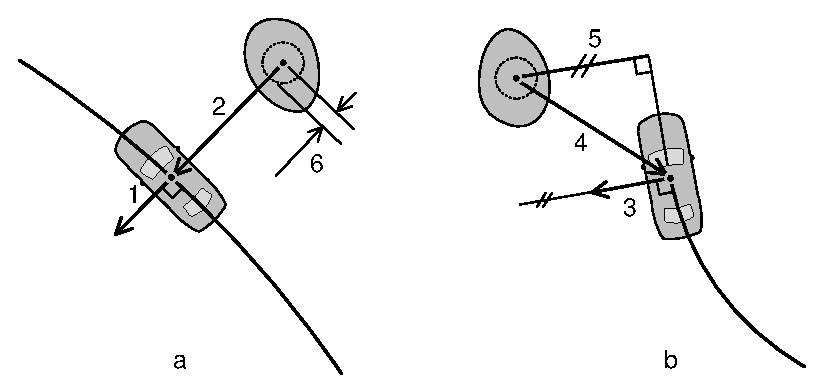
\includegraphics[width=1.0\textwidth,clip, trim = 0cm 0cm 0cm 0cm]{5_passingDirection}
    \caption[Restriktionen zur Vorgabe der Ausweichrichtung]{Restriktionen zur Vorgabe der Ausweichrichtung, vgl.\ auch \cite{gerdts2009generating}}
    \label{fig:skalarProduct}
    \end{center}
\end{figure}

\subsubsection{Wahl eines geeigneten Gütekriteriums\index{Gütekriterium}} \label{sec:costs}
Das Optimierungskriterium wird nachfolgend als Minimierung einer Kostenfunktion formuliert. Demnach dient sie als inverse Beschreibung des Idealverhaltens. Das Idealverhalten beim Ausweichmanöver ist wiederum charakterisiert durch eine maximale Reduktion der kinetischen Energie, d.h.\ Fahrzeuggeschwindigkeit, um bei einem dennoch auftretenden Fußgängerkontakt (weil er bspw.\ seinen Kurs spontan ändert) das geringste Verletzungspotential sicherzustellen. Darüber hinaus soll das Fahrzeug dem Fußgänger nicht zu nahe kommen, um Ungenauigkeiten in der Fußgängerdetektion und -prädiktion Rechnung zu tragen. Schließlich dürfen die Abweichungen weder in Position und Orientierung von der Referenzkurve noch die Lenkbewegungen zu groß sein, um einer allzu großen Irritation des Fahrers vorzubeugen. Diese verbalen Formulierungen werden nun nacheinander mathematisiert.

Zur Umsetzung der schnellstmöglichen Geschwindigkeitsreduktion wird nun gefordert, dass der Beschleunigungsvektor während des gesamten Manövers nicht nur innerhalb der Traktionsellipse, sondern genau auf dem Traktionsrand $[a_t/c_t]^2 + [a_n/c_n]^2 = 1$ liegt, da hierdurch bei gegebener Querbeschleunigung die maximal verfügbare Verzögerung realisiert wird. Die einfachste Berücksichtigung der Nebenbedingung ist das Auflösen nach $a_t:=\dot v = u_2$, sodass $u_2$ in \eqref{equ:vdot} ersetzt werden kann und daraus
\begin{align} \label{equ:replacement}
	\dot v = -c_t \sqrt{1-[v\dot\theta / c_n]^2}
\end{align}
resultiert. Demnach muss weder der Geschwindigkeitsreduktion im Kostenfunktional Rechnung getragen werden, noch eine Optimierung über das Eingangssignal $u_2$ stattfinden.

Die Zusammensetzung der Kostenfunktion $J$ wird nun in den anschließenden Abschnitten beleuchtet, wobei eine Aufteilung in einen bewegungsbezogenen und einen Fußgänger-bezogenen Term entsprechend
\begin{align}
\label{equ:totalcost}
	J(\vektor x, u_1) = J_{\text{mov}}(\vektor x, u_1) + J_{\text{ped}}(\vektor x)
\end{align}
vorgenommen wird.


\subsubsection{Bewegungskosten} \label{sec:costs_movement}
Zur Beschreibung der Idealbewegung innerhalb der eigenen Fahrspur wird nun
\begin{subequations}
\begin{align}
\label{equ:integralcosts}
	J_{\text{mov}}(\vektor x, u_1) = \int_{t_0}^{t_f}{\left\{u_1^2 + \!\!\!\!\!\!\!\!\! \sum_{i\in\{v,a,j,\theta,\kappa\}}\!\!\!\!\!\!\!\!\! k_i \,\, \Delta_i^2(\vektor x, u_1)\right\}\rm{d}t};  %+ k_{\text{ped}} \sum_{n=1}^N o(\min_{\tau\in [t_1,t_2]} \text{dist}_n(\tau))
\end{align}
\begin{align}
\label{equ:deltaV}
	\Delta_v(\vektor{x})		 			&= v[\theta-\theta_r],  & 
	\Delta_a(\vektor{x}) 				  &= v^2[\kappa-\kappa_r], 	 &
	\Delta_j(\vektor{x},u_1) 			&= v^2[\bar\kappa-\bar\kappa_r],\\
\label{equ:deltaTheta}
	\Delta_\theta(\vektor{x}) 		&= \theta - \theta_r, &
	\Delta_\kappa(\vektor{x}) 		&= \kappa - \kappa_r; 
	%\Delta_{\dot\delta}(x,u) &= u - \kappa_r'\dot s_r
\end{align}
\begin{align*}
\text{mit} \qquad \kappa := \frac{\delta}{l \left[ 1 + \left[\frac{v}{v_{\text{ch}}}\right]^2\right]}, 
\quad
\bar\kappa :=\diff{\kappa}{\delta}u_1,
%\bar\kappa := \frac{u_1}{l \left[ 1 + \left[\frac{v}{v_{\text{ch}}}\right]^2\right]},
\quad
\bar\kappa_r := \diff{\kappa_r}{s}\dot s
\end{align*}
\end{subequations}
definiert.  Hierbei bestrafen die Terme \eqref{equ:deltaV} die genäherte laterale Geschwindigkeit $\Delta_v \approx \dot d_r$, Beschleunigung $\Delta_a \approx \ddot d_r$ und den lateralen Ruck $\Delta_j \approx \dddot d_r$. Aufgrund der Multiplikation mit $v$ dominieren diese Ausdrücke die Trajektorienkosten bei höherer Längsgeschwindigkeit und sorgen für eine bestimmte Geschwindigkeitsinvarianz: Falls die Restriktionen während des Fahrmanövers nicht aktiv sind, werden die Passagiere (in einer äquivalenten Situation) dasselbe Beschleunigungsprofil bei $\unitfrac[10]{m}{s}$ wie bei  $\unitfrac[30]{m}{s}$ erfahren. Das wiederum bedeutet, dass eine aufwändige Parameteradaption über den gesamten Geschwindigkeitsbereich entfällt. \\
Bei niedrigen Geschwindigkeiten hingegen, kurz bevor das Fahrzeug zum Stehen kommt, verschwinden die Terme, weshalb die geometrisch motivierten Terme \eqref{equ:deltaTheta} ergänzt werden, die in Kombination mit dem Integral von $u_1^2$ in \eqref{equ:integralcosts} ein wohlgeartetes Lenkverhalten bis in den Stand sicherstellen.

Erwähnenswert ist, dass im Unterschied zu anderen Arbeiten auf einen Kostenterm für $d_r$ verzichtet wird. Grund hierfür ist, dass das Fahrzeug nach dem Ausweichmanöver nicht eigenständig zur Fahrbahnmitte zurückkehren darf, da sich hinter dem ersten noch weitere, undetektierte Fußgänger aufhalten können und darüber hinaus die Fahrerirritation zunimmt.


\subsubsection{Annäherungskosten für Fußgänger} \label{sec:costs_obstacles}
Auf die Berücksichtigung des detektierten Fußgängers (s.\ bspw.\ \cite{gandhi2007pedestrian}) %Sensorübersicht für Fußgängerausweichen
in den Integralkosten wird bewusst verzichtet, da das, wie in Abschn.\,\ref{sec:direkte_methode_kostenfuktional} erläutert, in vielen Situationen zu ungewollten Effekten führt. 
%Bspw. würde ein schnelles Vorbeifahren am Fußgänger zu geringeren Kosten führen als ein langsames. Das Skalieren der Kosten, z.B.\ um die Differenzgeschwindigkeit zum Fußgänger, resultiert in anderen Problemen, sodass 
Stattdessen wird der über den Optimierungshorizont prädizierte Mindestabstand $d_{\min } := \min d(t)$ des Fahrzeugumrisses zum Fußgänger in den Kosten berücksichtigt. Hierdurch ergibt sich
\begin{align*}
   J_{\text{ped}}(\vektor x) = k_{\text{ped}} \, C(d_{\min}(\vektor x)),
\end{align*}
wobei die Annäherung an den Fußgänger über die Funktion $C(\cdot) = [\min ([(\cdot)-d_{\text{infl}}],0)]^2$
bestraft wird, deren Parameter $d_{\text{infl}}$ den Einflussbereich der Kosten
entsprechend Abb.\,\ref{fig:distanceCosts} nach Erfahrungswerten
definiert. Neben dem geringen Rechenaufwand zeichnet sich die Funktion dadurch aus,
%Diese Funktion bietet folgende Vorteile. Im Vergleich zu einer linearen Kostenzunahme ist die Funktion um $d_{\text{infl}}$ herum stetig differenzierbar. Darüber hinaus hält sich der Rechenaufwand in Grenzen. Und schließlich sind die
dass die Kosten immer endlich sind, was wichtig für eine robuste Konvergenz des Optimierers ist. Schließlich ist eine korrekt geplante Kollisionsfolgenminderung einem physikalisch nicht realisierbarem Manöver vorzuziehen.

\begin{figure}[h]
        \psfrag{1}[cb][cb][1.0]{$d_{\min }$}
        \psfrag{2}[ct][ct][1.0]{$d_{\text{infl}}$}
				\psfrag{3}[r][r][1.0]{$C(d_{\min })$}
        \psfrag{4}[cb][cb][1.0]{$0$}
    \begin{center}
    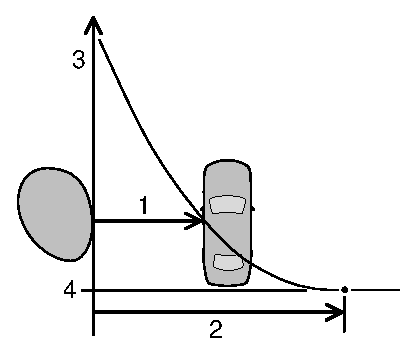
\includegraphics[width=0.5\textwidth,clip, trim = 0cm 0cm 0cm 0cm]{5_distanceCosts}
    \caption[Quadratischer Kostenanstieg in der Umgebung eines Hindernisses]{Quadratischer Kostenanstieg in der Umgebung eines Hindernisses; $d_{\text{infl}}$ zur Verdeutlichung vergrößert dargestellt \citeltex{werling2012cdc}}
    \label{fig:distanceCosts}
    \end{center}
\end{figure}

Damit ist das restringierte Optimalsteuerungsproblem genau definiert, sodass sich der nächste Abschnitt mit dessen Lösung auf Basis der direkten Optimierung beschäftigt. 

\subsection{Implementierung und Evaluation} \label{sec:implementation}
\label{sec:results} % Weil andere Section nicht mehr unterteilt wurde
Die Lösung des Optimalsteuerungsproblems erfolgt aufgrund der gutmütigen Systemeigenschaften des Prädiktionsmodells über das in Absch.\,\ref{sec:direkte_einfach_schiessverfahren} beschriebene Einfachschießverfahren. Hierbei wird die endliche Parametrierung des Eingangs $u_1$ klassisch über ein stückweise konstantes Eingangssignal vorgenommen (20 Stützstellen, Initialisierung mit dem Nullvektor) und die Differentialgleichung mittels Runge-Kutta erster Ordnung für den gewählten Prädiktionshorizont von $t_f - t_0 = \unit[2.0]{s}$ gelöst. Die Optimierung selbst übernimmt ein SQP-Verfahren \cite{papageorgiou2012optimierung}, wofür die benötigten Routinen in C implementiert werden.  % entsprechend der Übersicht in Abb.\,\ref{fig:solveOCP_ablaufplan} im Anhang
Die Wichtungsfaktoren werden zu $[k_v, k_a, k_j, k_\theta, k_\kappa]=[10^3, 10^2, 10^1, 10^2, 10^1, 10^0]$ gewählt (in SI-Einheiten), und der simulierte Fußgänger mit $d_{\text{infl}}=\unit[0.2]{m}$ und $k_\text{ped} = 10^5$ berücksichtigt. Die Fahrzeugprädiktion erfolgt mit $v_\text{ch}=\unitfrac[50]{km}{h}$, $\dot \delta_{\max} = - \dot \delta_{\min} = \unitfrac[0.8]{rad}{s}$,  $d_{\max} = -d_{\min} = \unit[2.0]{m}$ und $c_n=c_t=\unitfrac[10.0]{m}{s^2}$. \\
Insgesamt ergibt sich für das nichtlineare Programm auf einem i5-520M (2.4 $\unit[]{GHz}$) Prozessor eine Ausführungszeit von ca.\ $\unit[0.12]{s}$,   womit der Algorithmus grundsätzlich für eine Echtzeitanwendung im Fahrzeug geeignet ist, vgl. auch \cite{alamir2010use}. \\
%
Die optimale Lösung wird nun anhand der in Abb.\,\ref{fig:fussgaenger_draufsicht} dargestellten Situation beurteilt, in der der Fußgänger unmittelbar vor dem Fahrzeug auftaucht, sodass eine Kollision mit alleinigem Bremsen nicht mehr zu verhindern ist. Es sei angemerkt, dass das Hindernis hier lediglich aus Darstellungsgründen als stationär gewählt ist und keinerlei Einschränkungen bzgl.\ dynamischer Hindernisse bestehen, s.\ \citeltex{werling2012cdc}. Durch die Vorgabe von $\gamma = -1$ wird der Algorithmus zudem dazu veranlasst, nach links auszuweichen, ohne die Fahrspur zu verlassen. \\
Während des Manövers bremst das Fahrzeug so schnell wie möglich in den Stand, ohne die durch den Kamm'schen Kreis genäherte Fahrphysik zu überschreiten. Wie den dazugehörigen Signalverläufen in Abb.\,\ref{fig:fussgaenger_draufsicht_signale} zu entnehmen ist, zeichnet sich die optimale Trajektorie durch ein gleichmäßiges Ein- und Auslenken mit anschließendem Stabilisieren bis in den Stand aus. Aufgrund der gewählten Zielfunktion wird hierbei ein optimaler Kompromiss zwischen dem Sicherheitsabstand zum Fußgänger und der Eingriffsstärke der Lenkung gefunden. Auffällig ist zudem der Verzögerungsverlauf in Fahrzeuglängsrichtung (tangentiale Beschleunigung $a_t$), der sich durch die maximale quer-längs-kombinierte Kraftpotentialausnutzung ergibt. Das Fahrzeug öffnet also automatisch dann die Bremse, wenn die Querbeschleunigung zunimmt, sodass der Kamm'sche Kreis nicht überschritten wird, um ein Schleudern zu verhindern.


%
%Die optimierte Trajektorie wird wiederum in jedem Schritt an einen e/a-linearisierenden Regler weitergeleitet, welcher mit einer Zykluszeit von $\unit[0.01]{s}$ die eigentlichen Stellgrößen eines nichtlinearen Zweispurmodells liefert, das neben Sensorrauschen auch die dynamischen Aufstandskräfte sowie nichtlineare Kopplungseffekte der Reifen simuliert. \\


%\section{Simulative Validierung} 


%he top views of the simulation results are depicted by Fig.\,\ref{fig:exp_topview_1} through Fig.\,\ref{fig:exp_topview_3}. Here, the optimized trajectory $[x_1, x_2]^\T$ is represented by time-equidistant interconnected dots, the circle represents a pedestrian and the thick solid line its prediction on $T_\text{hor}$. On both sides of the vehicle the dashed lines mark the road boundaries, whereas the dash-dotted line serves as the reference curve. \\
%Right below, the optimized input signal $u_1$, the predicted steering angle $\delta$, and velocity $v$ are shown as time plots. Furthermore, in the lower left of each figure, the planned trajectory is projected into the acceleration plane $[a_n, a_t]$ within the $\unit[1.0]{g}$-friction circle drawn in black.\\ 
%In addition, the black arrow represents the desired acceleration vector forwarded to the feedback controller, whose $a_t$-component is the second system input $u_2$. These three depicted points in time are also marked as vertical, dashed lines in Fig.\,\ref{fig:exp_control_plots}, which shows the resulting closed-loop time signals of the steering angle $\delta_c$ and the velocity $v_c$ of the simulated car. Below can be found the desired acceleration values  $a_{td}, a_{nd}$ commanded to the feedback controller and the actual measurements $a_t,a_n$. \\


%Zu Simulationsbeginn bewegt sich das Fahrzeug mit $v=\unitfrac[17.0]{m}{s}$ entlang einer leicht gekrümmten Linkskurve, als plötzlich ein Fußgänger von rechts (s.\ Kreis in Abb.\,\ref{fig:results} oben links) die Fahrspur betritt. Seine prädizierte Trajektorie aktiviert daraufhin das automatische Kollisionsvermeidungssystem, welches den kombinierten Brems-Ausweich-Eingriff initiiert.
% Skript hier: C:\SVN\Funktionsentwicklung\Ausweichassistenz\Kollisionsvermeidung\Matlabimplementierung\Singleshooting\Singleshooting_statisch

\begin{figure}
	\centering
	\input{../bilder/5_AuswertungSingleshooting_szene}
	\renewcommand{\matlabtextA}{\scriptsize}
	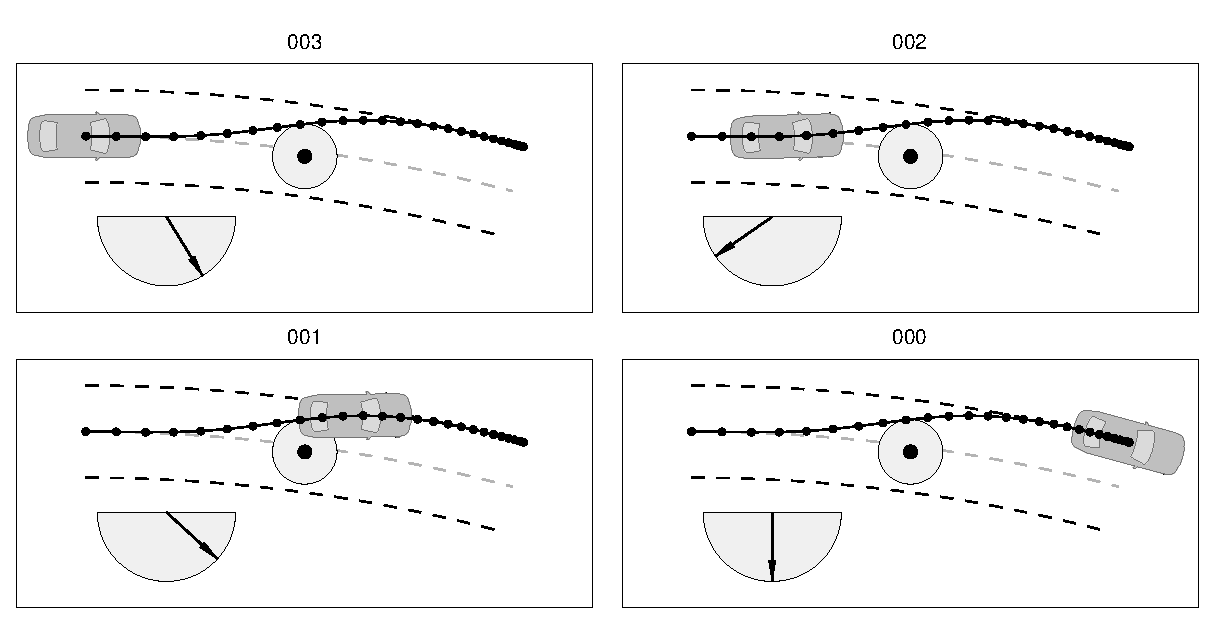
\includegraphics[width=1.0 \linewidth,trim = 0cm 0cm 0cm 0cm]{5_AuswertungSingleshooting_szene.eps}		
	%def\xlabel{$t$ in \unit{s}}
    \caption[Unfallvermeidung durch Bremsen und Ausweichen]{Ergebnis des Optimalsteuerungsproblems zur Vermeidung eines Fußgängerunfalls durch kombiniertes Bremsen und Ausweichen unter Ausnutzung des Kamm'schen Kreises \citeltex{werling2012cdc}.}
    \label{fig:fussgaenger_draufsicht}
\end{figure}
	
\begin{figure}	
\centering
	\def\xlabel{$t$ in $\unit{s}$}
	\def\ylabelA{$v$ in $\unitfrac{m}{s}$}	
	\def\ylabelB{$\delta$ in $\unit{rad}$}	
	\def\ylabelC{$u_1$ in $\unitfrac{rad}{s}$}
	\def\ylabelD{$a_t$ in $\unitfrac{m}{s^2}$}	
	\def\ylabelE{$a_n$ in $\unitfrac{m}{s^2}$}
	% Generated using matlabfrag
% Version: v0.6.16
% Version Date: 04-Apr-2010
% Author: Zebb Prime
%
%% <text>
%
\providecommand\matlabtextA{\color[rgb]{0.000,0.000,0.000}\fontsize{10}{10}\selectfont\strut}%
\psfrag{020}[tc][tc]{\matlabtextA \xlabel}%
\psfrag{021}[tc][tc]{\matlabtextA \ylabelA}%
\psfrag{022}[tc][tc]{\matlabtextA \ylabelD}%
\psfrag{023}[tc][tc]{\matlabtextA \ylabelE}%
\psfrag{024}[tc][tc]{\matlabtextA \ylabelB}%
\psfrag{025}[tc][tc]{\matlabtextA \ylabelC}%
%
%% </text>
%
%% <xtick>
%
\def\matlabfragNegXTick{\mathord{\makebox[0pt][r]{$-$}}}
%
\psfrag{000}[ct][ct]{\matlabtextA $0$}%
\psfrag{001}[ct][ct]{\matlabtextA $0.5$}%
\psfrag{002}[ct][ct]{\matlabtextA $1$}%
\psfrag{003}[ct][ct]{\matlabtextA $1.5$}%
\psfrag{004}[ct][ct]{\matlabtextA $2$}%
%
%% </xtick>
%
%% <ytick>
%
\psfrag{005}[rc][rc]{\matlabtextA $0$}%
\psfrag{006}[rc][rc]{\matlabtextA $10$}%
\psfrag{007}[rc][rc]{\matlabtextA $20$}%
\psfrag{008}[rc][rc]{\matlabtextA $-10$}%
\psfrag{009}[rc][rc]{\matlabtextA $0$}%
\psfrag{010}[rc][rc]{\matlabtextA $10$}%
\psfrag{011}[rc][rc]{\matlabtextA $-10$}%
\psfrag{012}[rc][rc]{\matlabtextA $0$}%
\psfrag{013}[rc][rc]{\matlabtextA $10$}%
\psfrag{014}[rc][rc]{\matlabtextA $-1$}%
\psfrag{015}[rc][rc]{\matlabtextA $0$}%
\psfrag{016}[rc][rc]{\matlabtextA $1$}%
\psfrag{017}[rc][rc]{\matlabtextA $-1$}%
\psfrag{018}[rc][rc]{\matlabtextA $0$}%
\psfrag{019}[rc][rc]{\matlabtextA $1$}%
%
%% </ytick>
	\renewcommand{\matlabtextA}{\normalsize }
  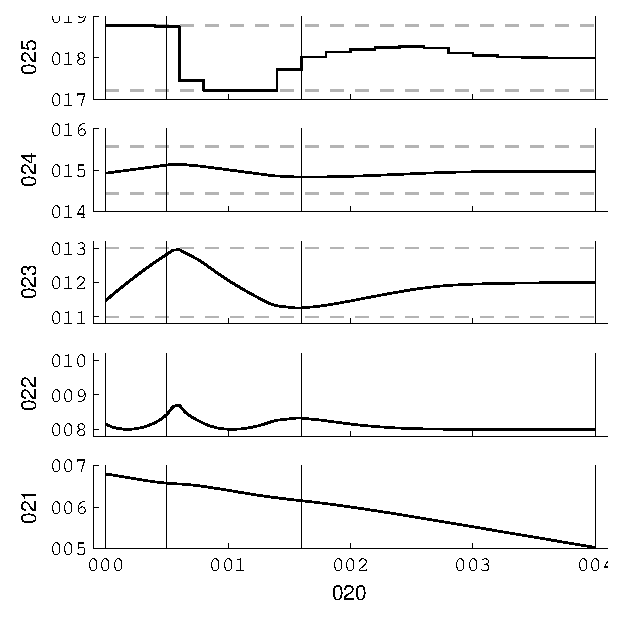
\includegraphics[width=1.0 \linewidth,trim = 0cm 0cm 0cm 0cm]{5_AuswertungSingleshooting_signals.eps}
    \caption[Signalverläufe bei kombiniertem Bremsen und Ausweichen]{Signalverläufe zu Abb.\,\ref{fig:fussgaenger_draufsicht} mit optimaler Steuerung $u_1$, Lenkwinkel $\delta$,  Quer- und Längsbeschleunigung $a_t, a_n$ sowie Geschwindigkeit $v$; Die vertikalen Linien markieren die Zeitpunkte der Draufsichten, die horizontalen gestrichelten Linien die Nebenbedingungen \citeltex{werling2012cdc}.}
    \label{fig:fussgaenger_draufsicht_signale}
	\end{figure}
	
	

%\begin{figure}[!h]
%\begin{minipage}[b]{0.48\linewidth}
%\centering
%\input{../bilder/5_fig_exp_topview_1.tex}
%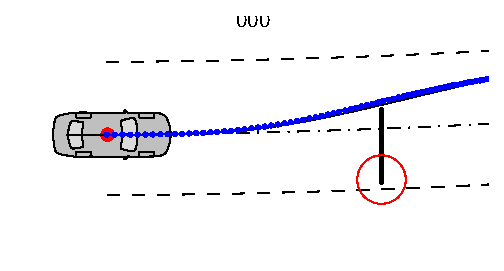
\includegraphics[width=1.0 \linewidth,trim = 0cm .5cm 0cm 0cm]{5_fig_exp_topview_1.eps}
%\input{../bilder/5_fig_exp_trajectory_plots_1.tex}
%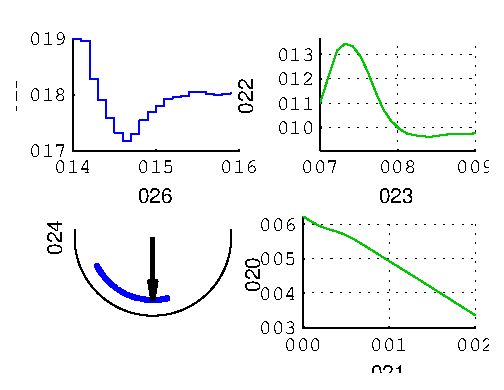
\includegraphics[width=.95 \linewidth]{5_fig_exp_trajectory_plots_1.eps}
%\vspace{.2cm}
%\end{minipage}
%\begin{minipage}[b]{0.48\linewidth}
%\centering
%\input{../bilder/5_fig_exp_topview_2.tex}
%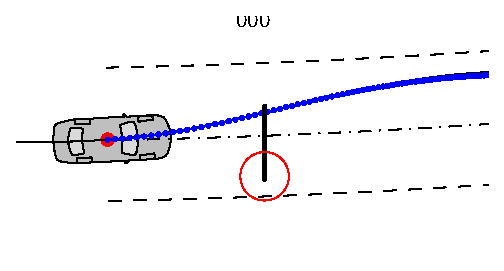
\includegraphics[width=1.0 \linewidth,trim = 0cm .5cm 0cm 0cm]{5_fig_exp_topview_2.eps}
%% Generated using matlabfrag
% Version: v0.6.16
% Version Date: 04-Apr-2010
% Author: Zebb Prime
%
%% <text>
%
\providecommand\matlabtextA{\color[rgb]{0.000,0.000,0.000}\fontsize{10}{10}\selectfont\strut}%
\psfrag{020}[bc][bc]{\matlabtextA $\unitfrac[v/]{m}{s}$}%
\psfrag{021}[tc][tc]{\matlabtextA $\unit[\tau/]{s}$}%
\psfrag{022}[bc][bc]{\matlabtextA $\unit[\delta/]{rad}$}%
\psfrag{023}[tc][tc]{\matlabtextA $\unit[\tau/]{s}$}%
\psfrag{024}[bc][bc]{\matlabtextA $u_2$}%
\psfrag{025}[bc][bc]{\matlabtextA $\unitfrac[u_1/]{rad}{s}$}%
\psfrag{026}[tc][tc]{\matlabtextA $\unit[\tau/]{s}$}%
%
%% </text>
%
%% <xtick>
%
\def\matlabfragNegXTick{\mathord{\makebox[0pt][r]{$-$}}}
%
\psfrag{000}[ct][ct]{\matlabtextA $0$}%
\psfrag{001}[ct][ct]{\matlabtextA $1$}%
\psfrag{002}[ct][ct]{\matlabtextA $2$}%
\psfrag{007}[ct][ct]{\matlabtextA $0$}%
\psfrag{008}[ct][ct]{\matlabtextA $1$}%
\psfrag{009}[ct][ct]{\matlabtextA $2$}%
\psfrag{014}[ct][ct]{\matlabtextA $0$}%
\psfrag{015}[ct][ct]{\matlabtextA $1$}%
\psfrag{016}[ct][ct]{\matlabtextA $2$}%
%
%% </xtick>
%
%% <ytick>
%
\psfrag{003}[rc][rc]{\matlabtextA $0$}%
\psfrag{004}[rc][rc]{\matlabtextA $5$}%
\psfrag{005}[rc][rc]{\matlabtextA $10$}%
\psfrag{006}[rc][rc]{\matlabtextA $15$}%
\psfrag{010}[rc][rc]{\matlabtextA $-0.05$}%
\psfrag{011}[rc][rc]{\matlabtextA $0$}%
\psfrag{012}[rc][rc]{\matlabtextA $0.05$}%
\psfrag{013}[rc][rc]{\matlabtextA $0.1$}%
\psfrag{017}[rc][rc]{\matlabtextA $-0.5$}%
\psfrag{018}[rc][rc]{\matlabtextA $0$}%
\psfrag{019}[rc][rc]{\matlabtextA $0.5$}%
%
%% </ytick>
%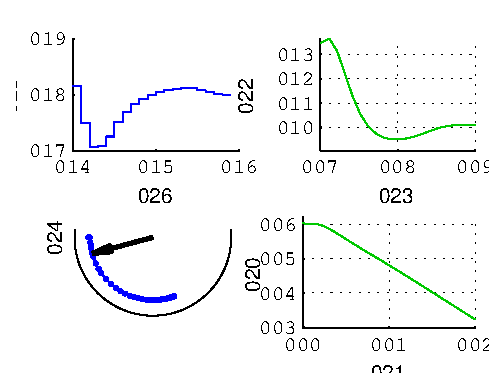
\includegraphics[width=.95 \linewidth]{5_fig_exp_trajectory_plots_2.eps}
%\vspace{.2cm}
%\end{minipage}
%\begin{minipage}[b]{0.48\linewidth}
%\centering
%\input{../bilder/5_fig_exp_topview_3.tex}
%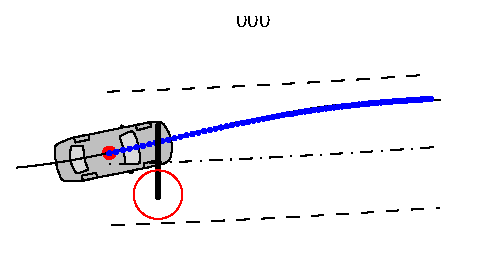
\includegraphics[width=1.0 \linewidth,trim = 0cm .5cm 0cm -1cm]{5_fig_exp_topview_3.eps}
%\input{../bilder/5_fig_exp_trajectory_plots_3.tex}
%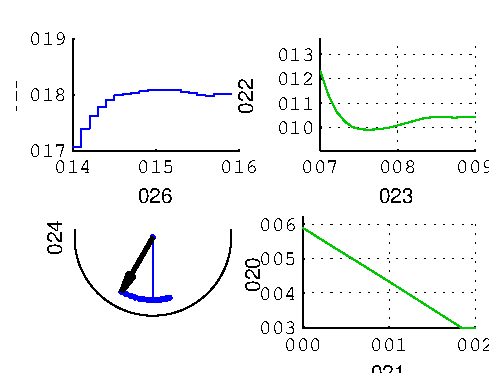
\includegraphics[width=1.0 \linewidth]{5_fig_exp_trajectory_plots_3.eps}
%\end{minipage}
%\begin{minipage}[b]{0.48\linewidth}
%\centering
%% Generated using matlabfrag
% Version: v0.6.16
% Version Date: 04-Apr-2010
% Author: Zebb Prime
%
%% <text>
%
\providecommand\matlabtextA{\color[rgb]{0.000,0.000,0.000}\fontsize{10}{10}\selectfont\strut}%
\psfrag{042}[bc][bc]{\matlabtextA $[a_n,a_{nd}]/\unitfrac{m}{s^2}$}%
\psfrag{043}[tc][tc]{\matlabtextA $\unit[t/]{s}$}%
\psfrag{044}[bc][bc]{\matlabtextA $[a_t,a_{td}]/\unitfrac{m}{s^2}$}%
\psfrag{045}[tc][tc]{\matlabtextA $\unit[t/]{s}$}%
\psfrag{046}[bc][bc]{\matlabtextA $\unitfrac[v_c /]{m}{s}$}%
\psfrag{047}[tc][tc]{\matlabtextA $\unit[t/]{s}$}%
\psfrag{048}[bc][bc]{\matlabtextA $\unit[\delta_c /]{rad}$}%
\psfrag{049}[tc][tc]{\matlabtextA $\unit[t/]{s}$}%
%
%% </text>
%
%% <xtick>
%
\def\matlabfragNegXTick{\mathord{\makebox[0pt][r]{$-$}}}
%
\psfrag{000}[ct][ct]{\matlabtextA $0$}%
\psfrag{001}[ct][ct]{\matlabtextA $0.5$}%
\psfrag{002}[ct][ct]{\matlabtextA $1$}%
\psfrag{003}[ct][ct]{\matlabtextA $1.5$}%
\psfrag{004}[ct][ct]{\matlabtextA $2$}%
\psfrag{005}[ct][ct]{\matlabtextA $2.5$}%
\psfrag{012}[ct][ct]{\matlabtextA $0$}%
\psfrag{013}[ct][ct]{\matlabtextA $0.5$}%
\psfrag{014}[ct][ct]{\matlabtextA $1$}%
\psfrag{015}[ct][ct]{\matlabtextA $1.5$}%
\psfrag{016}[ct][ct]{\matlabtextA $2$}%
\psfrag{017}[ct][ct]{\matlabtextA $2.5$}%
\psfrag{023}[ct][ct]{\matlabtextA $0$}%
\psfrag{024}[ct][ct]{\matlabtextA $0.5$}%
\psfrag{025}[ct][ct]{\matlabtextA $1$}%
\psfrag{026}[ct][ct]{\matlabtextA $1.5$}%
\psfrag{027}[ct][ct]{\matlabtextA $2$}%
\psfrag{028}[ct][ct]{\matlabtextA $2.5$}%
\psfrag{032}[ct][ct]{\matlabtextA $0$}%
\psfrag{033}[ct][ct]{\matlabtextA $0.5$}%
\psfrag{034}[ct][ct]{\matlabtextA $1$}%
\psfrag{035}[ct][ct]{\matlabtextA $1.5$}%
\psfrag{036}[ct][ct]{\matlabtextA $2$}%
\psfrag{037}[ct][ct]{\matlabtextA $2.5$}%
%
%% </xtick>
%
%% <ytick>
%
\psfrag{006}[rc][rc]{\matlabtextA $-2$}%
\psfrag{007}[rc][rc]{\matlabtextA $0$}%
\psfrag{008}[rc][rc]{\matlabtextA $2$}%
\psfrag{009}[rc][rc]{\matlabtextA $4$}%
\psfrag{010}[rc][rc]{\matlabtextA $6$}%
\psfrag{011}[rc][rc]{\matlabtextA $8$}%
\psfrag{018}[rc][rc]{\matlabtextA $-8$}%
\psfrag{019}[rc][rc]{\matlabtextA $-6$}%
\psfrag{020}[rc][rc]{\matlabtextA $-4$}%
\psfrag{021}[rc][rc]{\matlabtextA $-2$}%
\psfrag{022}[rc][rc]{\matlabtextA $0$}%
\psfrag{029}[rc][rc]{\matlabtextA $5$}%
\psfrag{030}[rc][rc]{\matlabtextA $10$}%
\psfrag{031}[rc][rc]{\matlabtextA $15$}%
\psfrag{038}[rc][rc]{\matlabtextA $-0.05$}%
\psfrag{039}[rc][rc]{\matlabtextA $0$}%
\psfrag{040}[rc][rc]{\matlabtextA $0.05$}%
\psfrag{041}[rc][rc]{\matlabtextA $0.1$}%
%
%% </ytick>
%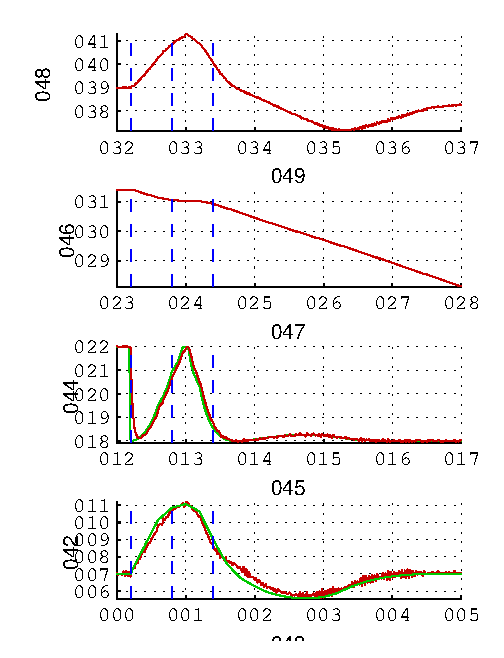
\includegraphics[width=1.0 \linewidth]{5_fig_exp_control_plots.eps}
%\end{minipage}
%\caption
%{Simulative Funktionsvalidierung mittels nichtlinearem längs-quer-gekoppeltem Zweispurmodell. Die optimierten Stellgrößen $u_1$ und $u_2$ bezeichnen die Lenkwinkelrate bzw.~ die Längsbeschleunigung. Der Lenkwinkel des vereinfachten Optimierungsmodells wird mit $\delta$ bezeichnet, die Fahrzeuggeschwindigkeit mit $v$. Der rote Kreis stellt die aktuelle Fußgängerposition einschl. Sicherheitsabstand dar. $()_c$ bezeichnet die wahren Fahrzeuggrößen.}
%\label{fig:results}
%\end{figure}

%Die Algorihmus zeigt folglich, wie mit aktiven Lenkeingriffen der gewonnene Freiheitsgrad dazu eingesetzt werden, Kollisionen mit Fußgängern zu verhindern, die mit alleinigem Bremsen nicht mehr vermeidbar sind. %Aus diesem Grund wurde auf Basis der NMPC eine Online-Planungsstrategie hergeleitet, welche den Besonderheiten der Anwendung Rechnung trägt. Diese beinhaltet die numerische Prädiktion eines einfachen, numerisch effizienten und dennoch hinreichend genauen Fahrzeugmodells, welches Beschleunigungs- und Lenkdynamikbeschränkungen unterliegt. Aufgrund der gewählten Zielfunktion wird ein optimaler Kompromiss zwischen dem Sicherheitsabstand zum Fußgänger und der Eingriffsstärke der Lenkung gefunden, was simulativ nachgewiesen wird. Die nächsten Schritte beinhalten die Laufzeitoptimierung mit anschließender Umsetzung der vorgeschlagenen Methodik auf einem Realfahrzeug unter Einbezug der Umfelderkennung.

\section{Bewertung}
Der Hauptvorteil der direkten Methode besteht darin, dass (im Unterschied zur indirekten Methode des nachfolgenden Kapitels) keine \emph{kanonischen Gleichungen} aufgestellt werden müssen. Das vereinfacht insbesondere die Systemmodellierung und die Zusammenstellung des Kostenfunktionals, da sie nur "`vorwärts"' programmiert werden müssen und das nichtlineare Programm die Lösung selbständig sucht. Bei der prototypischen Umsetzung neuer Fahrerassistenzfunktionen stellt sich zudem die direkte Optimierungsmethode als vergleichsweise flexibel heraus, da während des Entwicklungsprozesses eine bestehende Programmstruktur problemlos durch zusätzliche Kostenterme und Nebenbedingungen erweitert werden kann, um neue Erkenntnisse aus Simulationen und praktischen Fahrversuchen einfließen zu lassen. Überhaupt können Nebenbedingungen in Form von Zustandsbeschränkungen leichter berücksichtigt werden als bei der indirekten Methode. \\
Als großer Nachteil erweist sich die unmittelbare Abhängigkeit vom einzusetzenden statischen Optimierungsalgorithmus, dem sog.\ Solver\index{Solver}, der \iA nur \emph{lokal} konvergiert. Damit ist die Wahl der Startlösung des Optimierungsvektors ganz entscheidend für das Optimierungsergebnis und die dafür benötigte Zeit. Insbesondere kombinatorische Fahrmanöverprobleme (Einparken, Ausweichen zwischen mehreren Hindernisse hindurch etc.), können deshalb nur unzureichend adressiert werden, sodass das Verfahren für solche Anwendungen mit einer vorgelagerten Startlösungssuche basierend auf globalen Optimierungsmethoden der Dynamischen Programmierung des vorangegangenen Kapitels zu kombinieren ist. \\ %s.\ Kap.\,\ref{chap:dynamische_Optimierung_dynamisch}) und einem vereinfachten Systemmodell zu kombinieren ist. %, s.\ z.B.\ \cite{dolgov2010path, montemerlo2008junior}. \\
Auch wenn die Leistungsfähigkeit der Steuergeräte stetig zunimmt, so können sie den Rechenaufwand bei umfassenden Fahrzeugmodellen noch nicht in Echtzeit bewältigen. Dennoch stellt dann die direkte Optimierungsmethode eine hervorragende Möglichkeit dar, den Testfahrer in virtuellen Fahrversuchen zu ersetzen, sodass beispielsweise Fahrwerkseinstellungen bereits am virtuellen Fahrzeug beurteilt werden können.


% Hauptprobleme:
	%- Erfordernis eines NLP-Solvers, der abgesichert werden muss, Blackbox, erfodern nur ein grobes verständnis. Absicherung???
	%- Nachweis der Konvergenz schwierig, Startlösung erfoderlich, allerdings nicht für konjugierte Zustände, wie bei indirekter Optimierung.
	%- Laufzeit, falls Fahrzeugmodell aufwändig gewählt, dann nur offline (Für den Offlinebetrieb (LUT) und zur analyse ein hervorragendes mittel, auch für lattice und co.; Aufeinander folgende Probleme sind schneller zu lösen, da startlösung bekannt; analytische Jakobimatrix schwierig --> Forschungsbedarf
	%
		%- Multishooting: interessant bei mehrkernprozessoren auf steuergeräten.
%% Hauptvorteile:
	% Was sollen andere machen?

% TODO: noch weitere Verfahren namentlich erwähnen: collocation, Jakobimatrix


\cleardoublepage
